\documentclass[]{book}
\usepackage{lmodern}
\usepackage{amssymb,amsmath}
\usepackage{ifxetex,ifluatex}
\usepackage{fixltx2e} % provides \textsubscript
\ifnum 0\ifxetex 1\fi\ifluatex 1\fi=0 % if pdftex
  \usepackage[T1]{fontenc}
  \usepackage[utf8]{inputenc}
\else % if luatex or xelatex
  \ifxetex
    \usepackage{mathspec}
  \else
    \usepackage{fontspec}
  \fi
  \defaultfontfeatures{Ligatures=TeX,Scale=MatchLowercase}
\fi
% use upquote if available, for straight quotes in verbatim environments
\IfFileExists{upquote.sty}{\usepackage{upquote}}{}
% use microtype if available
\IfFileExists{microtype.sty}{%
\usepackage{microtype}
\UseMicrotypeSet[protrusion]{basicmath} % disable protrusion for tt fonts
}{}
\usepackage[margin=1in]{geometry}
\usepackage{hyperref}
\hypersetup{unicode=true,
            pdftitle={Data Science avec R},
            pdfauthor={Fousseynou Bah},
            pdfborder={0 0 0},
            breaklinks=true}
\urlstyle{same}  % don't use monospace font for urls
\usepackage{natbib}
\bibliographystyle{apalike}
\usepackage{color}
\usepackage{fancyvrb}
\newcommand{\VerbBar}{|}
\newcommand{\VERB}{\Verb[commandchars=\\\{\}]}
\DefineVerbatimEnvironment{Highlighting}{Verbatim}{commandchars=\\\{\}}
% Add ',fontsize=\small' for more characters per line
\usepackage{framed}
\definecolor{shadecolor}{RGB}{248,248,248}
\newenvironment{Shaded}{\begin{snugshade}}{\end{snugshade}}
\newcommand{\KeywordTok}[1]{\textcolor[rgb]{0.13,0.29,0.53}{\textbf{#1}}}
\newcommand{\DataTypeTok}[1]{\textcolor[rgb]{0.13,0.29,0.53}{#1}}
\newcommand{\DecValTok}[1]{\textcolor[rgb]{0.00,0.00,0.81}{#1}}
\newcommand{\BaseNTok}[1]{\textcolor[rgb]{0.00,0.00,0.81}{#1}}
\newcommand{\FloatTok}[1]{\textcolor[rgb]{0.00,0.00,0.81}{#1}}
\newcommand{\ConstantTok}[1]{\textcolor[rgb]{0.00,0.00,0.00}{#1}}
\newcommand{\CharTok}[1]{\textcolor[rgb]{0.31,0.60,0.02}{#1}}
\newcommand{\SpecialCharTok}[1]{\textcolor[rgb]{0.00,0.00,0.00}{#1}}
\newcommand{\StringTok}[1]{\textcolor[rgb]{0.31,0.60,0.02}{#1}}
\newcommand{\VerbatimStringTok}[1]{\textcolor[rgb]{0.31,0.60,0.02}{#1}}
\newcommand{\SpecialStringTok}[1]{\textcolor[rgb]{0.31,0.60,0.02}{#1}}
\newcommand{\ImportTok}[1]{#1}
\newcommand{\CommentTok}[1]{\textcolor[rgb]{0.56,0.35,0.01}{\textit{#1}}}
\newcommand{\DocumentationTok}[1]{\textcolor[rgb]{0.56,0.35,0.01}{\textbf{\textit{#1}}}}
\newcommand{\AnnotationTok}[1]{\textcolor[rgb]{0.56,0.35,0.01}{\textbf{\textit{#1}}}}
\newcommand{\CommentVarTok}[1]{\textcolor[rgb]{0.56,0.35,0.01}{\textbf{\textit{#1}}}}
\newcommand{\OtherTok}[1]{\textcolor[rgb]{0.56,0.35,0.01}{#1}}
\newcommand{\FunctionTok}[1]{\textcolor[rgb]{0.00,0.00,0.00}{#1}}
\newcommand{\VariableTok}[1]{\textcolor[rgb]{0.00,0.00,0.00}{#1}}
\newcommand{\ControlFlowTok}[1]{\textcolor[rgb]{0.13,0.29,0.53}{\textbf{#1}}}
\newcommand{\OperatorTok}[1]{\textcolor[rgb]{0.81,0.36,0.00}{\textbf{#1}}}
\newcommand{\BuiltInTok}[1]{#1}
\newcommand{\ExtensionTok}[1]{#1}
\newcommand{\PreprocessorTok}[1]{\textcolor[rgb]{0.56,0.35,0.01}{\textit{#1}}}
\newcommand{\AttributeTok}[1]{\textcolor[rgb]{0.77,0.63,0.00}{#1}}
\newcommand{\RegionMarkerTok}[1]{#1}
\newcommand{\InformationTok}[1]{\textcolor[rgb]{0.56,0.35,0.01}{\textbf{\textit{#1}}}}
\newcommand{\WarningTok}[1]{\textcolor[rgb]{0.56,0.35,0.01}{\textbf{\textit{#1}}}}
\newcommand{\AlertTok}[1]{\textcolor[rgb]{0.94,0.16,0.16}{#1}}
\newcommand{\ErrorTok}[1]{\textcolor[rgb]{0.64,0.00,0.00}{\textbf{#1}}}
\newcommand{\NormalTok}[1]{#1}
\usepackage{longtable,booktabs}
\usepackage{graphicx,grffile}
\makeatletter
\def\maxwidth{\ifdim\Gin@nat@width>\linewidth\linewidth\else\Gin@nat@width\fi}
\def\maxheight{\ifdim\Gin@nat@height>\textheight\textheight\else\Gin@nat@height\fi}
\makeatother
% Scale images if necessary, so that they will not overflow the page
% margins by default, and it is still possible to overwrite the defaults
% using explicit options in \includegraphics[width, height, ...]{}
\setkeys{Gin}{width=\maxwidth,height=\maxheight,keepaspectratio}
\IfFileExists{parskip.sty}{%
\usepackage{parskip}
}{% else
\setlength{\parindent}{0pt}
\setlength{\parskip}{6pt plus 2pt minus 1pt}
}
\setlength{\emergencystretch}{3em}  % prevent overfull lines
\providecommand{\tightlist}{%
  \setlength{\itemsep}{0pt}\setlength{\parskip}{0pt}}
\setcounter{secnumdepth}{5}
% Redefines (sub)paragraphs to behave more like sections
\ifx\paragraph\undefined\else
\let\oldparagraph\paragraph
\renewcommand{\paragraph}[1]{\oldparagraph{#1}\mbox{}}
\fi
\ifx\subparagraph\undefined\else
\let\oldsubparagraph\subparagraph
\renewcommand{\subparagraph}[1]{\oldsubparagraph{#1}\mbox{}}
\fi

%%% Use protect on footnotes to avoid problems with footnotes in titles
\let\rmarkdownfootnote\footnote%
\def\footnote{\protect\rmarkdownfootnote}

%%% Change title format to be more compact
\usepackage{titling}

% Create subtitle command for use in maketitle
\newcommand{\subtitle}[1]{
  \posttitle{
    \begin{center}\large#1\end{center}
    }
}

\setlength{\droptitle}{-2em}

  \title{Data Science avec R}
    \pretitle{\vspace{\droptitle}\centering\huge}
  \posttitle{\par}
    \author{Fousseynou Bah}
    \preauthor{\centering\large\emph}
  \postauthor{\par}
      \predate{\centering\large\emph}
  \postdate{\par}
    \date{2019-02-12}

\usepackage{booktabs}

\begin{document}
\maketitle

{
\setcounter{tocdepth}{1}
\tableofcontents
}
\chapter{Introduction}\label{introduction}

\section{\texorpdfstring{Un autre livre sur la \emph{data science}!
Vraiment?}{Un autre livre sur la data science! Vraiment?}}\label{un-autre-livre-sur-la-data-science-vraiment}

En décidant d'écrire un livre sur la \emph{data science}, j'ai
longuement débattu dans ma propre tête, je me suis posé plusieurs
questions dont une qui revenait constamment: ``a-t-on vraiment besoin
d'un autre livre sur la \emph{data science}?'' ``N'en-t-on pas assez?''
Avec le succès dont jouit la discipline, ce n'est certainement pas les
ressources qui manquent, aussi bien en ligne que dans les librairies. Et
surtout, je me demandais bien ``qu'avais-je à dire qui n'avait pas été
dit''? Et pourtant, quelques raisons m'ont poussé à reconsidérer ma
position.

La première est assez égoïte. On n'apprend jamais aussi bien qu'en
enseignant. Pour m'assurer que j'avais bien assimilé les connaissances
que j'avais acquises dans ce domaine, il n'y avait rien de mieux que de
me livrer à un exercice de pédagogue. Expliquer à d'autres ce que
j'avais appris. N'est-ce pas là que réside l'ultime test pour un
apprenant! C'est partant de cette idée que je me suis mis à faire des
diapositives dans le cadre des mes enseignements. Très tôt, j'ai réalisé
que les diapositives ne sauraient jouer leur rôle, qui est d'offrir un
aperçu synthétique d'une idée développée par un narrateur, et satifaire
l'apprenant qui souhaiterai obtenir des explications détaillées. Ce
travail revient au narrateur, à défaut de qui l'on se tourne vers un
manuel. Donc, il me fallait bien accompagner les diapositives d'un
support plus détaillé pour mieux outiller mes étudiants.

La seconde raison est le contexte. Malgré l'abondance et la qualité des
ressources disponibles sur la \emph{data science} et malgré l'accès de
plus en plus facile - coût faible et gratuité pour beaucoup -, il
demeure que l'étudiant africain peut souvent se sentir éloigné du
contexte à travers lequel la \emph{data science} est présentée. Or,
cell-ci est avant tout une discipline de contexte. Bien que mélangeant
informatique, mathématiques, statistiques\ldots{}et bien d'autres
expertises, elle est avant tout un outil, mobilisée pour répondre à des
questions. Et ces questions sont très contextuelles. Il ne fait aucun
doute que le disponibilité et l'accéssibilité des données sur le monde
industrialisé rend leur utilisation commode pour introduire la
\emph{data science} à un jeune africain est très commode. Mais la
distance entre le contexte présenté et celui qui est vécu par le
bénéficiaire pose un problème. Elle empêche l'appropriation de la
discipline. De ce fait, je me suis trouvé dans ce constat une raison de
m'engager dans ce projet et surtout de me forcer à utiliser des données
sur le contexte local. Après tout, l'être humain n'est-il pas plus
enclin à vous prêter attention quand vous lui parlez de lui-même?

\section{\texorpdfstring{La \emph{data
science}}{La data science}}\label{la-data-science}

Comme toute discipline qui connaît une expansion rapide, il est
difficile de définir la \emph{data science}. Elle est vaste et riche,
tant de par les disciplines dont elle emprunte des morceaux pour se
contituer en entité que de par les branches qu'elle pousse avec sa
propre croissance.

Commençons par quelques exemples

Fait de la \emph{data science}:

\begin{itemize}
\item
  l'économiste qui examine le niveau du PIB sur 30 ans et cherche à
  dégager des scénarii pour des futures évolutions;
\item
  le sociologue qui s'appuie le taux de natalité et le taux de
  participation des femmes au marché du travail pour comprendre
  l'évolution de la place de la femme dans la société;
\item
  le météorologue qui cherche à prédire la pluviométrie de la semaine à
  venir en modélisant les données historiques;
\item
  l'épidémiologue qui cartographie le taux de prévalence du paludisme
  pour appuyer un programme stratégique;
\item
  etc.
\end{itemize}

Le caractère transversale de la \emph{data science} apparait ici quand
on sait que ces individus sont de disciplines différentes et poursuivent
des questions tout aussi distantes les unes des autres. Et pourtant, les
données les réunissent tous. Ils ont chacun besoin de trouver dans
celles-ci un appui pour améliorer leur propre compréhension du phénomène
étudié, tester leurs hypothèses, fonder leurs recommandations ou
même\ldots{}reconforter leurs propres idées ou mieux s'armer pour
rejetter celles de leurs adversaires (les données ne sont aussi neutres
que celui qui les manipule!)

Selon
\href{https://en.wikipedia.org/wiki/Data_science}{\textcolor{blue}{Wikipédia}},
la \emph{data science} est un champ interdisciplinaire qui utilise les
méthode, processus, algorithmes et systèmes scientifiques pour extraire
des données - tant structurées que non structurées - des informations
utiles à la compréhension et à la prise de décision. De ce fait, elle
s'appuie sur diverses méthodes (mathématiques, statistiques,
informatiques, etc.) pour tirer des données une compréhension meilleure
de phénomènes d'intérêt.

\section{\texorpdfstring{Le \emph{data
scientist}}{Le data scientist}}\label{le-data-scientist}

Et le \emph{data scientist} dans tout ça? Il est apparait désormais
comme la perle rare. Un individu capable de parler aux hommes, aux
machines et aux données. Aux:

\begin{itemize}
\item
  hommes, il pose les questions auxquelles il a la charge d'offrir des
  réponses.
\item
  machines, il parle à travers des langages spécifiques (R, Python,
  Julia,\ldots{}), des langages qui ressemblent à bien d'égards à ceux
  avec lesquels il s'entretient avec les humains car ils sont basés sur
  des règles précises et sont vivants et évolutifs;
\item
  données, il applique des méthodes d'investigation où l'expérience,
  l'intuition, le sens artistique interviennent tout autant que la
  connaissance du domaine d'intervention. Dans les données disponibles,
  il cherche à séparer les bonnes des mauvaises, les utiles des
  nuisibles. A celles qu'il sélectionne, il cherche le bon format, la
  bonne structure. Sur celles qu'il retient, il teste des modèles, sans
  oublier la place importante de la visualisation à tous les niveaux.
  Bref, un vrai détective!
\end{itemize}

Face à la génération massive des données, le besoin de \emph{data
scientist} se fait pressant partout. De ce fait l'engouement ne manque
pas pour les jeunes désireux de se lancer. Mais le portrait de
super-homme généralement fait du \emph{data scientist} (ne cherchez pas
plus loin que les lignes d'en dessus!), l'on peut croire qu'il faut être
spécial pour embrasser la profession. Du tout! Celà dit, certaines
compétences sont utiles.

Alors, qu'est-ce qu'il faut pour être \emph{data scientist}?

\begin{itemize}
\item
  pas nécéssairement un diplôme avancé en mathématiques ou en
  statistiques\ldots{}quoiqu'il est utile de maîtriser des concepts de
  bases (les concepts algébriques comme le vecteur, la matrice,\ldots{}
  et les notions statistiques comme la moyenne, l'écart-type, etc.);
\item
  pas forcément un diplôme en informatique ou en
  programmation\ldots{}quoiqu'il est utile de connaître les notions de
  bases (qu'est-ce qu'un objet, un environnement? quels types d'objets
  peut-on manipuler dans un environnement donnée\ldots{}?);
\item
  une connaissance avérée dans un domaine spécifique dans lequel l'on
  peut soulever des questions, mobiliser des outils théoriques auxquels
  on confronte les résultats de l'analyse conduite sur les données;
\item
  un esprit curieux, quelle que soit l'avenue que l'on emprunte.
\end{itemize}

Vous pourrez avoir une meilleure idée en surfant sur le net (Google est
votre ami!)

\section{R}\label{r}

\subsection{Qu'est-ce que c'est que R?}\label{quest-ce-que-cest-que-r}

Voici basiquement ce que
\href{https://fr.wikipedia.org/wiki/R_(langage)}{Wikipédia} dit.
\href{http://r-project.org}{\textcolor{blue}{R}} est un langage de
programmation et un logiciel gratuit et libre. Il est surtout utilisé
pour le développement de programmes statistiques et des analyses de
données. Il gagne en popularité depuis quelques années avec l'émergence
de la \emph{data science} et du fait qu'il est gratuit et ouvert
(\emph{open-source}). R est née d'un projet de recherche mené par deux
chercheurs, Ross Ihaka et Robert Gentleman à l'université d'Auckland
(Nouvelle-Zélande) en 1993. En 1997 est mis en place le
\emph{Comprehension R Archive Network (CRAN)} qui centralise les
contributions au projet

Depuis le projet connaît une croissance soutenue, grâce à des
contributions de la part de milliers de personnes à travers le monde.

\subsection{Pourquoi R?}\label{pourquoi-r}

Pour un apprenti \emph{data scientist}, le choix du langage et/ou du
programme est une décision critique. Considérant le temps qu'il
investira en apprentissage et le retour qu'il espéra à travers
l'utilisation de ses nouvelles connaissances dans sa profession, il est
utile de considerer divers critères dont:

\begin{itemize}
\item
  l'accessibilité de l'outil en termes de coûts: tous les langages de
  programmation ne sont pas gratuits comme R! Certains
  coûtent\ldots{}chers mêmes ;
\item
  l'accessibilité du langage en termes de syntaxe: R est très
  compréhensible (surtout pour quelqu'un qui se retrouve un peu avec la
  langue anglaise);
\item
  la popularité du langage parmi les paires: tout le monde s'est mis à
  l'anglais, même dans les pays où ce n'est pas la langue dominante.
  N'est-ce pas? De la même façon, il est important pour le \emph{data
  scientist} d'embrasser un langage qui est aussi utilisé par ceux avec
  lesquels il sera amené à collaborer. A ce niveau, R est très
  populaire.
\item
  la dynamique de développement du langage: le langage étant un
  investissement en soit, il est important de miser sur ceux qui
  présentent un avenir. Et ceux-ci sont ceux qui mutent avec la
  technologie et les besoins des utilisateurs. A ce niveau encore, R
  présente des arguments. Il dispose du réseau \emph{CRAN} alimenté par
  des milliers de contributeurs, divers aussi bien de par leur position
  dans le monde que de par leur discipline.
\end{itemize}

\subsection{R dans l'écosystème des
langages}\label{r-dans-lecosysteme-des-langages}

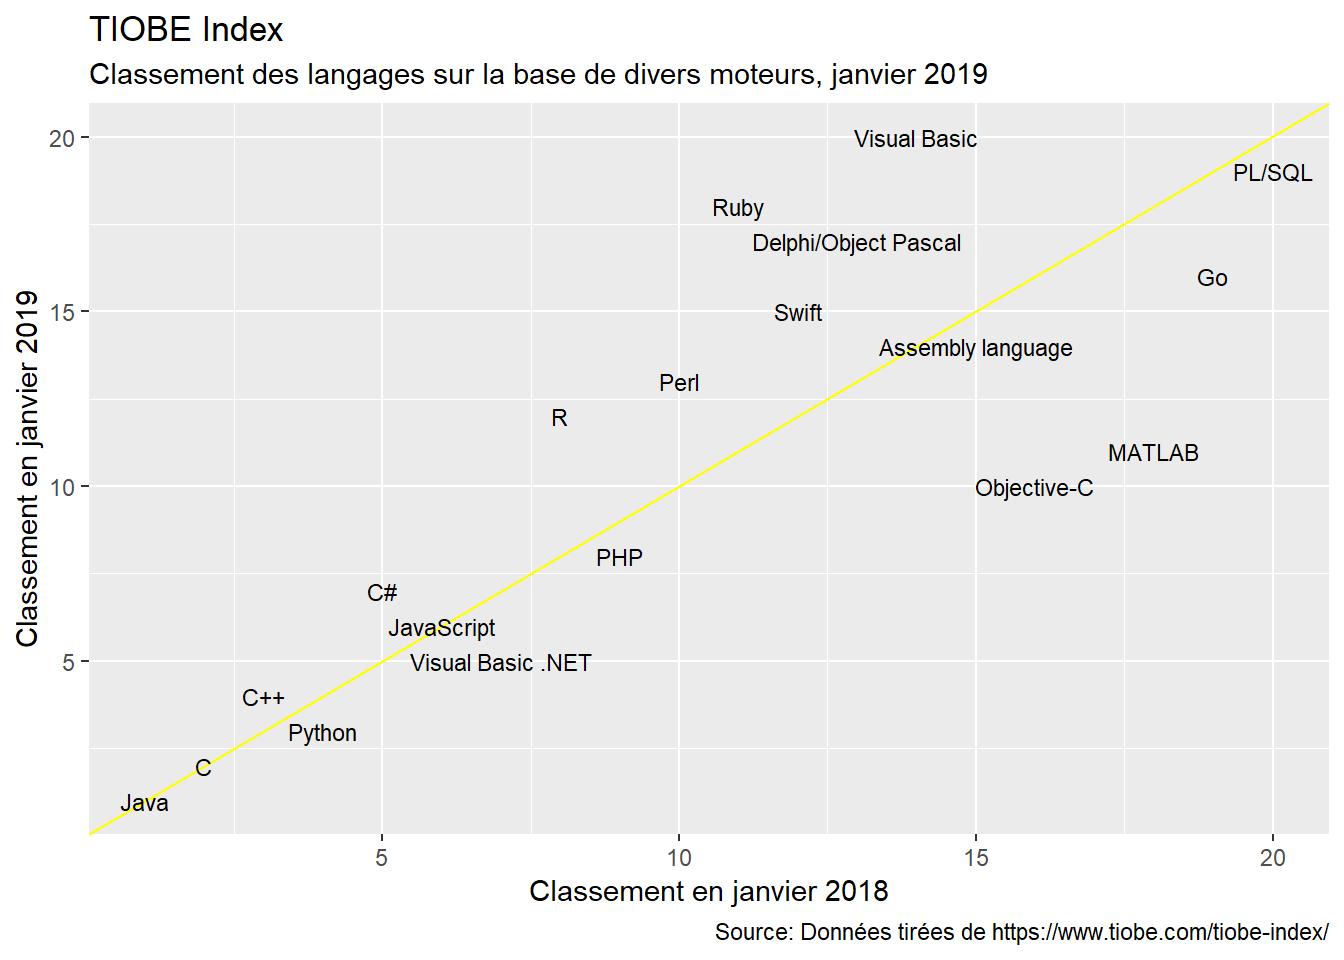
\includegraphics[width=1\linewidth,height=1\textheight]{dswr_book_files/figure-latex/unnamed-chunk-3-1}

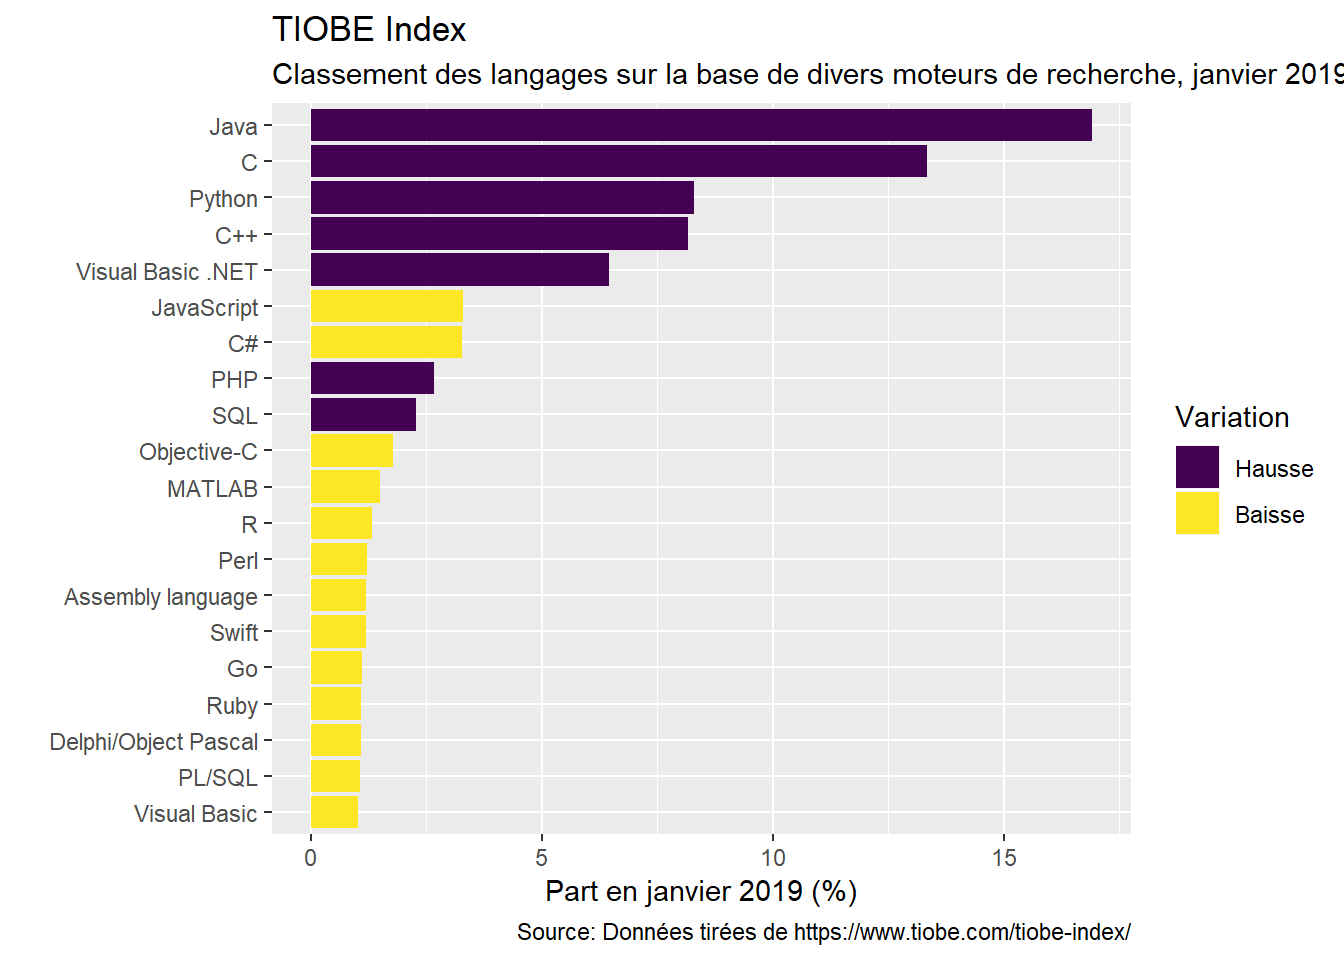
\includegraphics[width=1\linewidth,height=1\textheight]{dswr_book_files/figure-latex/unnamed-chunk-4-1}

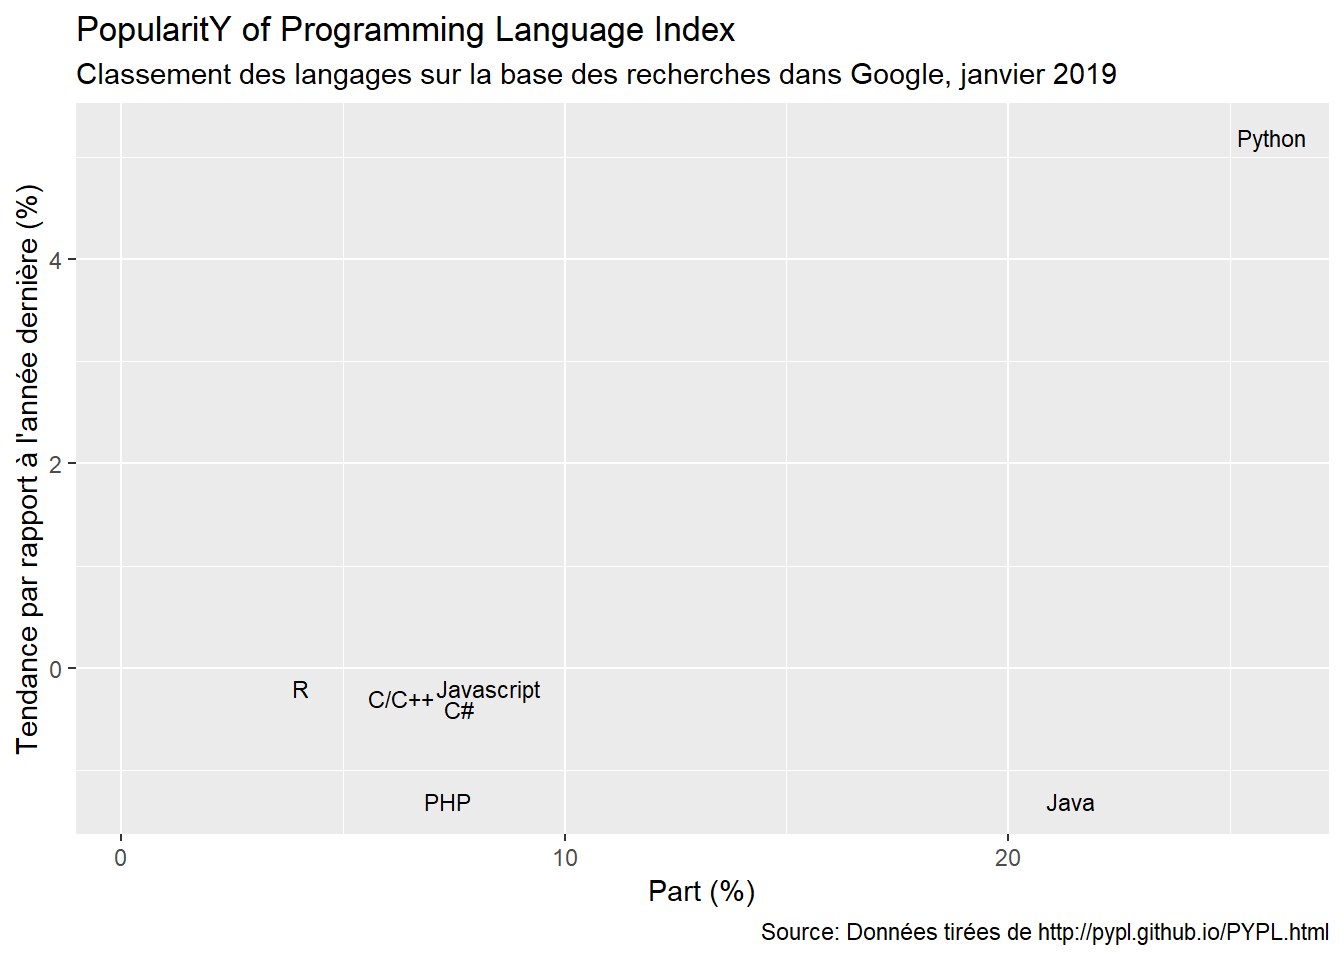
\includegraphics[width=1\linewidth,height=1\textheight]{dswr_book_files/figure-latex/unnamed-chunk-5-1}

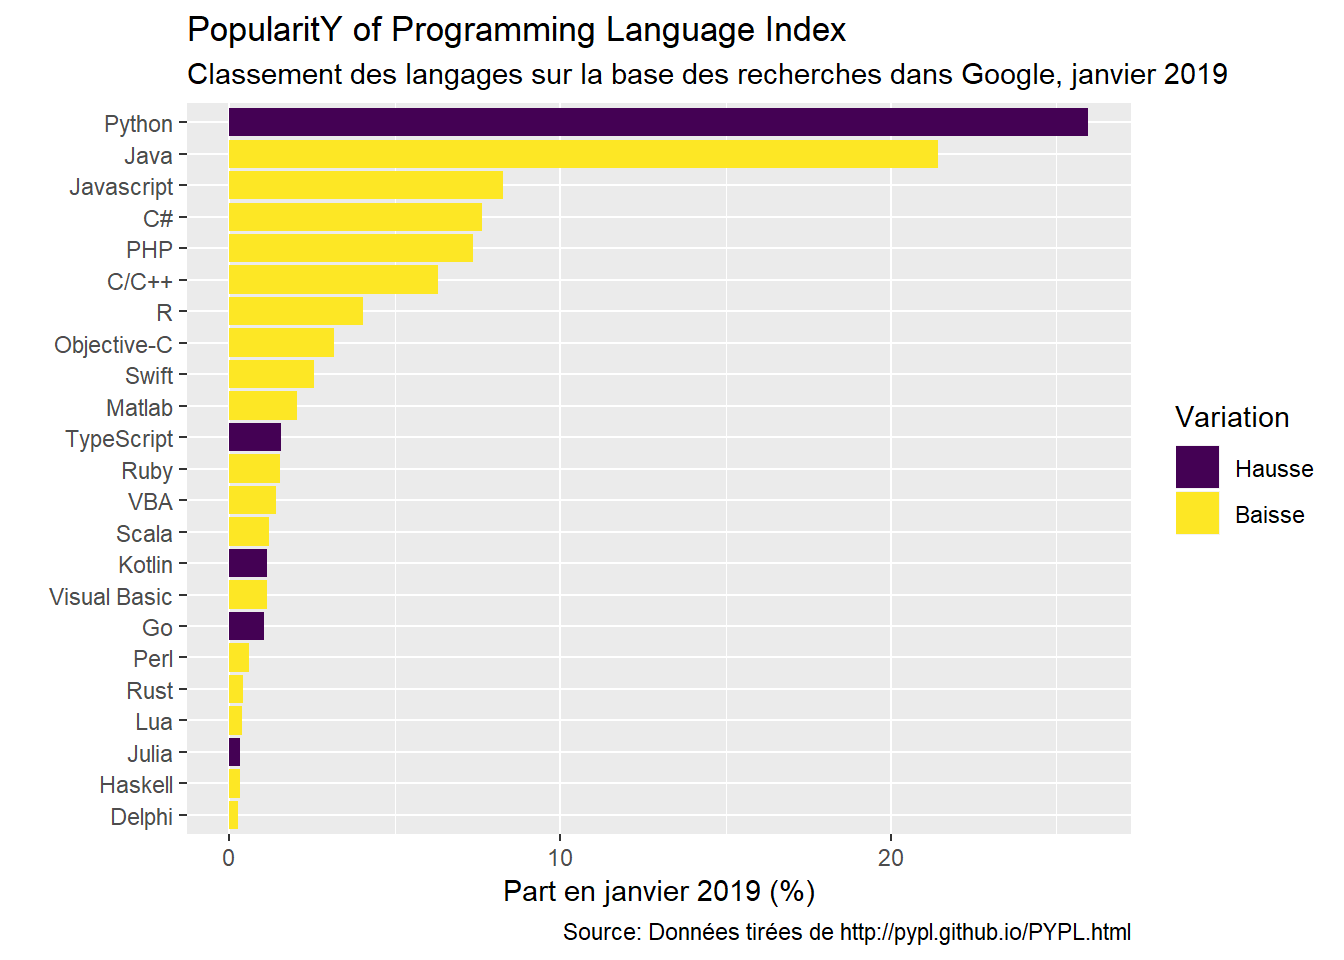
\includegraphics[width=1\linewidth,height=1\textheight]{dswr_book_files/figure-latex/unnamed-chunk-6-1}

Ce qui apparait des différentes figures, c'est que R parvient à se
tailler une place parmi les langages les plus populaires au monde. Et
celà, malgré le fait que c'est une langage spécialisée. Si sur les dix
dernières années, le langage s'est enrichi avec la diversification de
ses contributeurs, il reste à la base un langage élaboré par des
statisticiens pour des statisticiens. De ce fait, il est excéllent pour
l'analyse de données, mais fort peu utile pour certaines
tâches\ldots{}comme le développement d'un site web.

\section{RStudio}\label{rstudio}

\subsection{Qu'est-ce que c'est que
RStudio}\label{quest-ce-que-cest-que-rstudio}

\begin{itemize}
\item
  C'est une IDE (\emph{Integrated Development Environment}) ou
  Environnement Intégré de Développement
\item
  Il sert d'interface entre R et l'utilisateur, offre à celui diverses
  commodités d'utilisation
\end{itemize}

Maintenant, vous avez les outils nécéssaires pour commencer la
formidable aventuRe!

\chapter{Objets dans R}\label{objets-dans-r}

\section{Objectifs et outils}\label{objectifs-et-outils}

Dans ce chapitre, nous allons :

\begin{itemize}
\item
  introduire la notion d'objet dans R;
\item
  présenter un certain nombre d'entre eux;
\item
  et illustrer avec quelques exemples.
\end{itemize}

Que nous faudra-t-il?

\begin{itemize}
\item
  R (évidemment)
\item
  RStudio (de préférence)
\end{itemize}

\section{La notion d'objet dans R}\label{la-notion-dobjet-dans-r}

\subsection{Qu'est-ce qu'un objet?}\label{quest-ce-quun-objet}

Dans R, un objet représente un concept, une idée. Il se matérialise par
une entité qui possède sa propre identité. Dans celle-ci, l'on compte
deux aspects majeurs:

\begin{itemize}
\item
  la structure interne;
\item
  le comportement.
\end{itemize}

Illustrons pour comprendre. Commençons par créer des objets.

Imaginez que vous voulez créer et conserver des bouts d'information dans
R sur les présidents qui se sont succédés à la tête de la République du
Mali. Commençons par le premier président,
\href{https://fr.wikipedia.org/wiki/Modibo_Ke\%C3\%AFta_(1915-1977)}{Mobido
Keïta}. Créeons des objects relatifs à son nom et son prénom.

\begin{Shaded}
\begin{Highlighting}[]
\NormalTok{nom <-}\StringTok{ "Keïta"}
\NormalTok{prenom <-}\StringTok{ "Mobido"}
\end{Highlighting}
\end{Shaded}

L'acte d'assignation d'une valeur à un objet se fait par le signe
\texttt{\textless{}-} qui est équivalent à \texttt{=}. Chez beaucoup
d'utilisateurs, la préférence est donnée à la première. Ceci peut se
comprendre par le fait qu'avec \texttt{\textless{}-}, l'acte
d'assignation se différencie plus facilement d'autres utilisations du
signe \texttt{=} (dont notamment à l'intérieur de fonctions). Désormais,
ces informations sont stockées dans notre environnement. Pour vérifier
appellons-les! Ceci revient à les saisir dans notre console et à taper
``Entrée''!

\begin{Shaded}
\begin{Highlighting}[]
\NormalTok{nom}
\end{Highlighting}
\end{Shaded}

\begin{verbatim}
## [1] "Keïta"
\end{verbatim}

\begin{Shaded}
\begin{Highlighting}[]
\NormalTok{prenom}
\end{Highlighting}
\end{Shaded}

\begin{verbatim}
## [1] "Mobido"
\end{verbatim}

\subsection{Oranges et bananes}\label{oranges-et-bananes}

Enrichissons notre environnement des objets additionnels. Ajoutons
l'année d'accession au pouvoir. Appelons cet objet
\texttt{annee\_arrivee\_pouvoir}.

\begin{Shaded}
\begin{Highlighting}[]
\NormalTok{annee_arrivee_pouvoir <-}\StringTok{ }\DecValTok{1960}
\end{Highlighting}
\end{Shaded}

Comme pour les objets précédent, celui-ci aussi peut être invoqué:

\begin{Shaded}
\begin{Highlighting}[]
\NormalTok{annee_arrivee_pouvoir}
\end{Highlighting}
\end{Shaded}

\begin{verbatim}
## [1] 1960
\end{verbatim}

A l'instar de l'orange et de la banane, fort différentes bien que toutes
les deux des fruits, ici aussi nos objets diffèrent. Peut-on les
additionner?

\begin{Shaded}
\begin{Highlighting}[]
\NormalTok{nom }\OperatorTok{+}\StringTok{ }\NormalTok{annee_arrivee_pouvoir}
\end{Highlighting}
\end{Shaded}

\begin{verbatim}
## Error in nom + annee_arrivee_pouvoir: non-numeric argument to binary operator
\end{verbatim}

Non, en l'occurence! On a un message d'erreur. R, c'est comme la vraie
vie! Les oranges et les bananes ne se mélangent.

\subsection{Ce qui se ressemblent
s'assemblent}\label{ce-qui-se-ressemblent-sassemblent}

Les choses qui diffèrent ne s'assemblent pas Illustration d'une
propriété des objets: le comportement. Regardons les choses qui
marchent.

\begin{verbatim}
## [1] 2
\end{verbatim}

Maintenant stockons ce résultat dans un objet.

\begin{Shaded}
\begin{Highlighting}[]
\NormalTok{objet1 <-}\StringTok{ }\DecValTok{1} \OperatorTok{+}\StringTok{ }\DecValTok{1}
\end{Highlighting}
\end{Shaded}

Créons-en un autre.

\begin{Shaded}
\begin{Highlighting}[]
\NormalTok{objet2 <-}\StringTok{ }\DecValTok{2} \OperatorTok{+}\StringTok{ }\DecValTok{2}
\end{Highlighting}
\end{Shaded}

Amusons à faire diverses opérations avec ces deux objets

\begin{Shaded}
\begin{Highlighting}[]
\NormalTok{objet1 }\OperatorTok{+}\StringTok{ }\NormalTok{objet2}
\end{Highlighting}
\end{Shaded}

\begin{verbatim}
## [1] 6
\end{verbatim}

\begin{Shaded}
\begin{Highlighting}[]
\NormalTok{objet1 }\OperatorTok{-}\StringTok{ }\NormalTok{objet2}
\end{Highlighting}
\end{Shaded}

\begin{verbatim}
## [1] -2
\end{verbatim}

\begin{Shaded}
\begin{Highlighting}[]
\NormalTok{objet1 }\OperatorTok{*}\StringTok{ }\NormalTok{objet2}
\end{Highlighting}
\end{Shaded}

\begin{verbatim}
## [1] 8
\end{verbatim}

\begin{Shaded}
\begin{Highlighting}[]
\NormalTok{objet1 }\OperatorTok{/}\StringTok{ }\NormalTok{objet2}
\end{Highlighting}
\end{Shaded}

\begin{verbatim}
## [1] 0.5
\end{verbatim}

Bref, vous voyez l'idée! Les propriétés des objets déterminent les
intéractions auxquelles elles se prêtent. Et ce sont justement ces
intéractions qui constituent le coeur de l'analyse de données. D'où
l'importance de la notion d'objet.

\subsection{Quelques objets dans R}\label{quelques-objets-dans-r}

Dans R, l'on distingue plusieurs types d'objets. Nous en retiendrons ici
5, qui nous serons utiles tout le long de l'ouvrage. Il s'agit des:

\begin{itemize}
\item
  caractères (\emph{strings} en anglais);
\item
  nombres (entiers ou réels);
\item
  dates;
\item
  valeurs logiques qui ne prennent que deux valeurs: \texttt{TRUE}
  (vrai) ou \texttt{FALSE} (faux);
\item
  facteurs qui sont un format spécial dans R prévu pour les variables
  catégorielles.
\end{itemize}

Revenons à notre exemple \emph{présidentiel}! Nous avons déjà le nom et
le prénom\ldots{}

\begin{Shaded}
\begin{Highlighting}[]
\CommentTok{# Caractères}
\NormalTok{nom <-}\StringTok{ "Keïta"}
\NormalTok{prenom <-}\StringTok{ "Mobido"}
\end{Highlighting}
\end{Shaded}

\ldots{}ainsi que l'année d'arrivée au pouvoir.

\begin{Shaded}
\begin{Highlighting}[]
\CommentTok{# Nombre}
\NormalTok{annee_arrivee_pouvoir <-}\StringTok{ }\DecValTok{1960}
\end{Highlighting}
\end{Shaded}

Ajoutons la date de naissance,

\begin{Shaded}
\begin{Highlighting}[]
\CommentTok{# Date}
\NormalTok{date_naissance <-}\StringTok{ }\KeywordTok{as.Date}\NormalTok{(}\StringTok{"1915-06-04"}\NormalTok{)}
\end{Highlighting}
\end{Shaded}

une valeur logique indiquant s'il a eu un parcours militaire ou pas,

\begin{Shaded}
\begin{Highlighting}[]
\CommentTok{# Valeur logique}
\NormalTok{parcours_militaire <-}\StringTok{ }\OtherTok{FALSE}
\end{Highlighting}
\end{Shaded}

et enfin la région de naissance.

\begin{Shaded}
\begin{Highlighting}[]
\CommentTok{# Facteur}
\NormalTok{region_naissance <-}\StringTok{ }\KeywordTok{as.factor}\NormalTok{(}\StringTok{"Bamako"}\NormalTok{)}
\end{Highlighting}
\end{Shaded}

\subsection{La notion de classe et de
type}\label{la-notion-de-classe-et-de-type}

Quand on a faire à des objets dont on ignore l'identité, l'on peut
s'appuyer la fonction \texttt{class}. Celle-ci permeet de connaître la
classe de l'objet. La classe est un attribut qui contribue à la
formation de l'idée d'un objet. ``Avec quoi se mélange-t-il?'' ``A
quelles règles de transformation se soumet-il?'' Basiquement, la classe
dicte les principes régissant la manipulation de cet objet. Testons la
fonction sur les objets que nous venons de créer pour bien confirmer les
identités qu'on leur a attribuées.

\begin{Shaded}
\begin{Highlighting}[]
\KeywordTok{class}\NormalTok{(nom)}
\end{Highlighting}
\end{Shaded}

\begin{verbatim}
## [1] "character"
\end{verbatim}

\begin{Shaded}
\begin{Highlighting}[]
\KeywordTok{class}\NormalTok{(prenom)}
\end{Highlighting}
\end{Shaded}

\begin{verbatim}
## [1] "character"
\end{verbatim}

\begin{Shaded}
\begin{Highlighting}[]
\KeywordTok{class}\NormalTok{(annee_arrivee_pouvoir)}
\end{Highlighting}
\end{Shaded}

\begin{verbatim}
## [1] "numeric"
\end{verbatim}

\begin{Shaded}
\begin{Highlighting}[]
\KeywordTok{class}\NormalTok{(date_naissance)}
\end{Highlighting}
\end{Shaded}

\begin{verbatim}
## [1] "Date"
\end{verbatim}

\begin{Shaded}
\begin{Highlighting}[]
\KeywordTok{class}\NormalTok{(parcours_militaire)}
\end{Highlighting}
\end{Shaded}

\begin{verbatim}
## [1] "logical"
\end{verbatim}

\begin{Shaded}
\begin{Highlighting}[]
\KeywordTok{class}\NormalTok{(region_naissance)}
\end{Highlighting}
\end{Shaded}

\begin{verbatim}
## [1] "factor"
\end{verbatim}

Nous voyons que les résultats sont bien conformes aux dénominations que
nous leur avons données plus haut.

Dans R, il y a aussi la fonction \texttt{typeof} (ou \texttt{mode}, mais
nous resterons avec la première) qui permet de connaître le mode de
stockage d'un objet. Testons!

\begin{Shaded}
\begin{Highlighting}[]
\KeywordTok{typeof}\NormalTok{(nom)}
\end{Highlighting}
\end{Shaded}

\begin{verbatim}
## [1] "character"
\end{verbatim}

\begin{Shaded}
\begin{Highlighting}[]
\KeywordTok{typeof}\NormalTok{(prenom)}
\end{Highlighting}
\end{Shaded}

\begin{verbatim}
## [1] "character"
\end{verbatim}

\begin{Shaded}
\begin{Highlighting}[]
\KeywordTok{typeof}\NormalTok{(annee_arrivee_pouvoir)}
\end{Highlighting}
\end{Shaded}

\begin{verbatim}
## [1] "double"
\end{verbatim}

\begin{Shaded}
\begin{Highlighting}[]
\KeywordTok{typeof}\NormalTok{(date_naissance)}
\end{Highlighting}
\end{Shaded}

\begin{verbatim}
## [1] "double"
\end{verbatim}

\begin{Shaded}
\begin{Highlighting}[]
\KeywordTok{typeof}\NormalTok{(parcours_militaire)}
\end{Highlighting}
\end{Shaded}

\begin{verbatim}
## [1] "logical"
\end{verbatim}

\begin{Shaded}
\begin{Highlighting}[]
\KeywordTok{typeof}\NormalTok{(region_naissance)}
\end{Highlighting}
\end{Shaded}

\begin{verbatim}
## [1] "integer"
\end{verbatim}

Si pour les objets \texttt{nom} et \texttt{prenom} qui sont des lettres,
la classe et le type se confondent, la question est tout autre pour
d'autres objets. Regardons \texttt{region\_naissance}, par exemple. En
termes de classe, c'est un facteur. Par contre, en terme de type, R l'a
coercé en entier (\emph{integer}).

Les types sont assez génériques car présentant pratiquement les mêmes
nomenclatures d'un langage à un autre. Dans R, nous allons plus nous
intéressér aux types suivants:

\begin{itemize}
\item
  logique (\emph{logical});
\item
  entier (\emph{integer});
\item
  réel (\emph{double});
\item
  caractère (\emph{character});
\item
  liste (\emph{list});
\item
  valeur nulle (\emph{NULL}).
\end{itemize}

Les objets que nous avons vus là peuvent être pensés comme des briques.
Ils entrent à leur tour dans la formation d'autres objets qui varient
les uns des autres. Tout comme les constructions peuvent différer entre
elles.

\subsection{Vers d'autres types
d'objets}\label{vers-dautres-types-dobjets}

La deuxième catégorie d'objets que nous allons voir ici peuvent être
pensés comme des objets composites. Nous en verrons quatre types:

\begin{itemize}
\item
  le vecteur;
\item
  la matrice;
\item
  le \emph{data frame} (cadre de données ou données rectangulaires);
\item
  la liste.
\end{itemize}

\section{Vecteurs}\label{vecteurs}

\subsection{Qu'est-ce qu'un vecteur?}\label{quest-ce-quun-vecteur}

De façon très simple, un vecteur est un ensemble d'éléments de même
nature. Revenons à notre exemple pour mieux comprendre. Nous avons
défini l'objet \texttt{nom}, n'est-ce pas? Est-ce un vecteur? A quoi
peut-on voir si c'est un vecteur ou pas? La réponse:

\begin{Shaded}
\begin{Highlighting}[]
\KeywordTok{is.vector}\NormalTok{(nom)}
\end{Highlighting}
\end{Shaded}

\begin{verbatim}
## [1] TRUE
\end{verbatim}

Donc nous avons crééé des vecteurs depuis longtemps et on voit qu'un
objet d'un seul élément peut être un vecteur. Maintenant, compte le
nombre d'éléments que compte ce vecteur.

\begin{Shaded}
\begin{Highlighting}[]
\KeywordTok{length}\NormalTok{(nom)}
\end{Highlighting}
\end{Shaded}

\begin{verbatim}
## [1] 1
\end{verbatim}

C'est vraiment un singleton qu'on a là\ldots{}pour le moment!

\subsection{Créons-en, des vecteurs!}\label{creons-en-des-vecteurs}

Décidons d'étendre nos observations à tous les présidents de la
République du Mali. En voici de quoi nous faire revisiter nos livres
d'histoire\ldots{}ou juste visiter Wikipedia!

\begin{Shaded}
\begin{Highlighting}[]
\CommentTok{# Omettons les périodes de transition (la valeur pédagogique est ce qui est recherché ici!)}
\NormalTok{nom <-}\StringTok{ }\KeywordTok{c}\NormalTok{(}\StringTok{"Keïta"}\NormalTok{, }\StringTok{"Traoré"}\NormalTok{, }\StringTok{"Konaré"}\NormalTok{, }\StringTok{"Touré"}\NormalTok{, }\StringTok{"Keïta"}\NormalTok{)}
\NormalTok{prenom <-}\StringTok{ }\KeywordTok{c}\NormalTok{(}\StringTok{"Modibo"}\NormalTok{, }\StringTok{"Moussa"}\NormalTok{, }\StringTok{"Alpha Oumar"}\NormalTok{, }\StringTok{"Amadou Toumani"}\NormalTok{, }\StringTok{"Ibrahim Boubacar"}\NormalTok{)}
\NormalTok{date_naissance <-}\StringTok{ }\KeywordTok{as.Date}\NormalTok{(}\KeywordTok{c}\NormalTok{(}\StringTok{"1915-06-04"}\NormalTok{, }\StringTok{"1936-09-25"}\NormalTok{, }\StringTok{"1946-02-02"}\NormalTok{, }\StringTok{"1948-11-04"}\NormalTok{, }\StringTok{"1945-01-29"}\NormalTok{))}
\NormalTok{region_naissance <-}\StringTok{ }\KeywordTok{as.factor}\NormalTok{(}\KeywordTok{c}\NormalTok{(}\StringTok{"Bamako"}\NormalTok{, }\StringTok{"Kayes"}\NormalTok{, }\StringTok{"Kayes"}\NormalTok{, }\StringTok{"Mopti"}\NormalTok{, }\StringTok{"Koutiala"}\NormalTok{))}
\NormalTok{annee_arrivee_pouvoir <-}\StringTok{ }\KeywordTok{c}\NormalTok{(}\DecValTok{1960}\NormalTok{, }\DecValTok{1968}\NormalTok{, }\DecValTok{1992}\NormalTok{, }\DecValTok{2002}\NormalTok{, }\DecValTok{2013}\NormalTok{)}
\NormalTok{parcours_militaire <-}\StringTok{ }\KeywordTok{c}\NormalTok{(}\OtherTok{FALSE}\NormalTok{, }\OtherTok{TRUE}\NormalTok{, }\OtherTok{FALSE}\NormalTok{, }\OtherTok{TRUE}\NormalTok{, }\OtherTok{FALSE}\NormalTok{)}
\end{Highlighting}
\end{Shaded}

Maintenant, expérimentons! Commençons avec \texttt{nom} que nous avons
écrasé avec de nouvelles valeurs.

\begin{Shaded}
\begin{Highlighting}[]
\KeywordTok{is.vector}\NormalTok{(nom)}
\end{Highlighting}
\end{Shaded}

\begin{verbatim}
## [1] TRUE
\end{verbatim}

\begin{Shaded}
\begin{Highlighting}[]
\KeywordTok{length}\NormalTok{(nom)}
\end{Highlighting}
\end{Shaded}

\begin{verbatim}
## [1] 5
\end{verbatim}

\begin{Shaded}
\begin{Highlighting}[]
\KeywordTok{class}\NormalTok{(nom)}
\end{Highlighting}
\end{Shaded}

\begin{verbatim}
## [1] "character"
\end{verbatim}

\begin{Shaded}
\begin{Highlighting}[]
\KeywordTok{typeof}\NormalTok{(nom)}
\end{Highlighting}
\end{Shaded}

\begin{verbatim}
## [1] "character"
\end{verbatim}

``nom'' est un \textbf{vecteur}, un ensemble de \textbf{5} éléments en
\textbf{charactères}. Amusez-vous à expérimenter avec les autres
vecteurs.

\subsection{Vrai pour un, vrai pour
plusieurs}\label{vrai-pour-un-vrai-pour-plusieurs}

Vous vous rappelez que plus haut, nous voyions que les opérations
n'étaient pas possible entre de différentes natures. Et bien, cette
règle, valable à l'échelle des objets élémentaires, l'est aussi aux
échelles supérieures.

Prenons nos données et cherchons à déterminer l'âge des présidents à
leur arrivée au pouvoir. On a les éléments nécéssaires pour ce faire, la
date de naissance et l'année d'arrivée au pouvoir. Toutefois, ces deux
vecteurs ne sont pas de même nature.

\begin{Shaded}
\begin{Highlighting}[]
\NormalTok{age_arrivee_pouvoir <-}\StringTok{ }\NormalTok{annee_arrivee_pouvoir }\OperatorTok{-}\StringTok{ }\NormalTok{date_naissance}
\end{Highlighting}
\end{Shaded}

\begin{verbatim}
## Error in `-.Date`(annee_arrivee_pouvoir, date_naissance): can only subtract from "Date" objects
\end{verbatim}

On a un message d'erreur. Apparemment l'opération n'est pas possible. Il
faudrait procéder à une transformation: déduire de la date de naissance
l'année pour conduire l'opération avec celle-ci.

\begin{Shaded}
\begin{Highlighting}[]
\NormalTok{annee_naissance <-}\StringTok{ }\KeywordTok{as.numeric}\NormalTok{(}\KeywordTok{format}\NormalTok{(date_naissance,}\StringTok{'%Y'}\NormalTok{))}
\end{Highlighting}
\end{Shaded}

Testons si le nouveau vecteur est de même nature de celui de
\texttt{annee\_arrivee\_pouvoir}.

\begin{Shaded}
\begin{Highlighting}[]
\KeywordTok{class}\NormalTok{(annee_naissance)}
\end{Highlighting}
\end{Shaded}

\begin{verbatim}
## [1] "numeric"
\end{verbatim}

Maintenant, nous pouvons procéder à l'opération

\begin{Shaded}
\begin{Highlighting}[]
\NormalTok{age_arrivee_pouvoir <-}\StringTok{ }\NormalTok{annee_arrivee_pouvoir }\OperatorTok{-}\StringTok{ }\NormalTok{annee_naissance}
\NormalTok{age_arrivee_pouvoir}
\end{Highlighting}
\end{Shaded}

\begin{verbatim}
## [1] 45 32 46 54 68
\end{verbatim}

On le confirme: les oranges et les bananes ne se mélangent pas.
Toutefois, R nous fait souvent des cocktails de fruits en coerçant
certains éléments. Imaginons que l'on veuille rassembler le prénom et le
nom dans un seul vecteur. Collons avec une fonction de base dans R,
\texttt{paste}, (ne vous en faites pas, vous ferez progressivement
connaissance avec les fonctions!)

\begin{Shaded}
\begin{Highlighting}[]
\NormalTok{prenom_nom <-}\StringTok{ }\KeywordTok{paste}\NormalTok{(prenom, nom)}
\NormalTok{prenom_nom}
\end{Highlighting}
\end{Shaded}

\begin{verbatim}
## [1] "Modibo Keïta"           "Moussa Traoré"         
## [3] "Alpha Oumar Konaré"     "Amadou Toumani Touré"  
## [5] "Ibrahim Boubacar Keïta"
\end{verbatim}

On peut être enclin à dire que ceci est passé sans souci parce que
\texttt{nom} et \texttt{prenom} sont tous les deux des vecteurs en
caractères. Maintenant, et si l'on ajoutait l'année d'arrivée au
pouvoir?

\begin{Shaded}
\begin{Highlighting}[]
\NormalTok{prenom_nom_age <-}\StringTok{ }\KeywordTok{paste}\NormalTok{(prenom, nom, }\StringTok{","}\NormalTok{, age_arrivee_pouvoir)}
\NormalTok{prenom_nom_age}
\end{Highlighting}
\end{Shaded}

\begin{verbatim}
## [1] "Modibo Keïta , 45"           "Moussa Traoré , 32"         
## [3] "Alpha Oumar Konaré , 46"     "Amadou Toumani Touré , 54"  
## [5] "Ibrahim Boubacar Keïta , 68"
\end{verbatim}

C'est passé comme une lettre à la poste (pour la génération email, voici
ce qu'est \href{https://fr.wikipedia.org/wiki/Poste}{la poste}). Car R a
une hiérarchie entre les objets. Avant de déclarer forfait avec un
message d'erreur, il tente tant bien que mal d'exécuter l'opération. Sur
la base de cette hiérarchie, il coerce certains éléments à se conformer
à d'autres, partant du plus flexible au moins flexible: \texttt{logique}
\textless{} \texttt{entier} \textless{} \texttt{réel} \textless{}
\texttt{caractère}. Pour comprendre ça, créons un vecteur de valeurs
logiques.

\begin{Shaded}
\begin{Highlighting}[]
\NormalTok{vecteur_logique <-}\StringTok{ }\KeywordTok{c}\NormalTok{(}\OtherTok{TRUE}\NormalTok{, }\OtherTok{FALSE}\NormalTok{)}
\end{Highlighting}
\end{Shaded}

Confirmons sa classe.

\begin{Shaded}
\begin{Highlighting}[]
\KeywordTok{class}\NormalTok{(vecteur_logique)}
\end{Highlighting}
\end{Shaded}

\begin{verbatim}
## [1] "logical"
\end{verbatim}

Ajoutons un troisième élément qui sera un entier. Disons 1.

\begin{Shaded}
\begin{Highlighting}[]
\NormalTok{vecteur_entier <-}\StringTok{ }\KeywordTok{c}\NormalTok{(vecteur_logique, }\DecValTok{1}\NormalTok{)}
\end{Highlighting}
\end{Shaded}

Qu'obtenons-nous?

\begin{Shaded}
\begin{Highlighting}[]
\NormalTok{vecteur_entier}
\end{Highlighting}
\end{Shaded}

\begin{verbatim}
## [1] 1 0 1
\end{verbatim}

Des entiers! R a coercé \texttt{TRUE} en 1 et \texttt{FALSE} en 0.

\begin{Shaded}
\begin{Highlighting}[]
\KeywordTok{class}\NormalTok{(vecteur_entier)}
\end{Highlighting}
\end{Shaded}

\begin{verbatim}
## [1] "numeric"
\end{verbatim}

Ajoutons un quatrième élément, cette fois-ci une réel: 2.5 (dans R,
comme en anglais, les décimales viennent après un \texttt{.}, pas une
\texttt{,}, qui sert plutôt de séparateur de milliers).

\begin{Shaded}
\begin{Highlighting}[]
\NormalTok{vecteur_reel <-}\StringTok{ }\KeywordTok{c}\NormalTok{(vecteur_entier, }\FloatTok{2.5}\NormalTok{)}
\NormalTok{vecteur_reel}
\end{Highlighting}
\end{Shaded}

\begin{verbatim}
## [1] 1.0 0.0 1.0 2.5
\end{verbatim}

\begin{Shaded}
\begin{Highlighting}[]
\KeywordTok{class}\NormalTok{(vecteur_reel)}
\end{Highlighting}
\end{Shaded}

\begin{verbatim}
## [1] "numeric"
\end{verbatim}

La mutation se voit au fait que R a affecté aux trois premiers éléments
des décimales, bien qu'initialement c'étaient des entiers. Maintenant,
ajoutons un cinquième élément: un prénom.

\begin{Shaded}
\begin{Highlighting}[]
\NormalTok{vecteur_caractere <-}\StringTok{ }\KeywordTok{c}\NormalTok{(vecteur_reel, }\StringTok{"Mariam"}\NormalTok{)}
\NormalTok{vecteur_caractere}
\end{Highlighting}
\end{Shaded}

\begin{verbatim}
## [1] "1"      "0"      "1"      "2.5"    "Mariam"
\end{verbatim}

\begin{Shaded}
\begin{Highlighting}[]
\KeywordTok{class}\NormalTok{(vecteur_caractere)}
\end{Highlighting}
\end{Shaded}

\begin{verbatim}
## [1] "character"
\end{verbatim}

Là aussi, la coercion se voit.

\subsection{Nommer les éléments d'un
vecteur}\label{nommer-les-elements-dun-vecteur}

Jusque là, ce sont des objets à part intégrale que nous avons nommés. On
les a assignés des noms pour les garder dans notre environnement de
travail. Maintenant, nous allons donner un nom aux éléments de vecteur.
Dressons l'analogie suivante. Notre environnement dans R est comme une
rue. Dans celle-ci, nous avons des concessions dont les portes sont
toutes numérotées: ce sont les noms des objets. A l'intérieur des
concessions, nous avons des individus: ce sont les éléments à
l'intérieur de nos objets. Tout comme ces individus portent des prénoms,
nous pouvons donner des appélations aux éléments contenus dans nos
objets.

Considerons que nous voulons associer à chaque date de naissance le nom
du président en question.

\begin{Shaded}
\begin{Highlighting}[]
\KeywordTok{names}\NormalTok{(date_naissance) <-}\StringTok{ }\NormalTok{prenom_nom}
\end{Highlighting}
\end{Shaded}

Voyons ce que ça donne

\begin{Shaded}
\begin{Highlighting}[]
\NormalTok{date_naissance}
\end{Highlighting}
\end{Shaded}

\begin{verbatim}
##           Modibo Keïta          Moussa Traoré     Alpha Oumar Konaré 
##           "1915-06-04"           "1936-09-25"           "1946-02-02" 
##   Amadou Toumani Touré Ibrahim Boubacar Keïta 
##           "1948-11-04"           "1945-01-29"
\end{verbatim}

C'est beau non! Il est intéréssant de noter que quand on conduit des
opérations sur des vecteurs aux éléments nommés, le résultat peut
hériter de ces propriétés. Reprenons l'opération de déduction de l'âge à
l'arrivée au pouvoir. Rappelons les deux vecteurs.

\begin{Shaded}
\begin{Highlighting}[]
\NormalTok{annee_naissance}
\end{Highlighting}
\end{Shaded}

\begin{verbatim}
## [1] 1915 1936 1946 1948 1945
\end{verbatim}

\begin{Shaded}
\begin{Highlighting}[]
\NormalTok{annee_arrivee_pouvoir}
\end{Highlighting}
\end{Shaded}

\begin{verbatim}
## [1] 1960 1968 1992 2002 2013
\end{verbatim}

Nommons juste un des deux vecteurs.

\begin{Shaded}
\begin{Highlighting}[]
\KeywordTok{names}\NormalTok{(annee_naissance) <-}\StringTok{ }\NormalTok{prenom_nom}
\NormalTok{annee_naissance}
\end{Highlighting}
\end{Shaded}

\begin{verbatim}
##           Modibo Keïta          Moussa Traoré     Alpha Oumar Konaré 
##                   1915                   1936                   1946 
##   Amadou Toumani Touré Ibrahim Boubacar Keïta 
##                   1948                   1945
\end{verbatim}

Procédons à l'opération.

\begin{Shaded}
\begin{Highlighting}[]
\NormalTok{age_arrivee_pouvoir <-}\StringTok{ }\NormalTok{annee_arrivee_pouvoir }\OperatorTok{-}\StringTok{ }\NormalTok{annee_naissance}
\NormalTok{age_arrivee_pouvoir}
\end{Highlighting}
\end{Shaded}

\begin{verbatim}
##           Modibo Keïta          Moussa Traoré     Alpha Oumar Konaré 
##                     45                     32                     46 
##   Amadou Toumani Touré Ibrahim Boubacar Keïta 
##                     54                     68
\end{verbatim}

Le vecteur \texttt{age\_arrivee\_pouvoir} a hérité des noms d'éléments.

Cette règle n'est pas toutefois immuable. Quand les éléments sont
coercés à prendre une autre classe que leur classe de départ, ils
peuvent perdre leur nom, qui n'est qu'un de leurs attributs (qui sont
subordonnés à leur classe). Reprenons la déduction de l'année de
naissance à partir de la date de naissance.

\begin{Shaded}
\begin{Highlighting}[]
\NormalTok{annee_naissance <-}\StringTok{ }\KeywordTok{format}\NormalTok{(date_naissance,}\StringTok{'%Y'}\NormalTok{)}
\NormalTok{annee_naissance}
\end{Highlighting}
\end{Shaded}

\begin{verbatim}
##           Modibo Keïta          Moussa Traoré     Alpha Oumar Konaré 
##                 "1915"                 "1936"                 "1946" 
##   Amadou Toumani Touré Ibrahim Boubacar Keïta 
##                 "1948"                 "1945"
\end{verbatim}

\begin{Shaded}
\begin{Highlighting}[]
\KeywordTok{class}\NormalTok{(annee_naissance)}
\end{Highlighting}
\end{Shaded}

\begin{verbatim}
## [1] "character"
\end{verbatim}

Ici, l'année n'a pas été coercé. Elle a été extraite par la fonction
sous format de caractères. En voulant conformer le vecteur à la classe
de nombre (on descend dans la hiérarchie), on coerce les éléments.

\begin{Shaded}
\begin{Highlighting}[]
\NormalTok{annee_naissance <-}\StringTok{ }\KeywordTok{as.numeric}\NormalTok{(}\KeywordTok{format}\NormalTok{(date_naissance,}\StringTok{'%Y'}\NormalTok{))}
\NormalTok{annee_naissance}
\end{Highlighting}
\end{Shaded}

\begin{verbatim}
## [1] 1915 1936 1946 1948 1945
\end{verbatim}

\begin{Shaded}
\begin{Highlighting}[]
\KeywordTok{class}\NormalTok{(annee_naissance)}
\end{Highlighting}
\end{Shaded}

\begin{verbatim}
## [1] "numeric"
\end{verbatim}

Avec la coercion, les noms se perdent. Il est donc utile de se rappeler
que les noms d'éléments ne sont pas immunes à la coercion. Toutefois,
quand les opérations se passent entre des éléments de même nature, les
noms sont bien saufs!

\subsection{Opérations sur vecteurs}\label{operations-sur-vecteurs}

\subsubsection{Sélection explicite}\label{selection-explicite}

Il arrive souvent qu'on ne soit intéréssée que par un élément précis
d'un vecteur. Peut-être l'on souhaite connaître seulement l'âge du
premier président lors de son accès au pouvoir. C'est le premier élément
du vecteur \texttt{age\_arrivee\_pouvoir}.

\begin{Shaded}
\begin{Highlighting}[]
\NormalTok{age_arrivee_pouvoir[}\DecValTok{1}\NormalTok{]}
\end{Highlighting}
\end{Shaded}

\begin{verbatim}
## Modibo Keïta 
##           45
\end{verbatim}

Peut-être nous voulons l'information pour le 1er et le 3ème présidents.
Ce sont les 1er et 3ème éléments du vecteur.

\begin{Shaded}
\begin{Highlighting}[]
\NormalTok{age_arrivee_pouvoir[}\KeywordTok{c}\NormalTok{(}\DecValTok{1}\NormalTok{, }\DecValTok{3}\NormalTok{)]}
\end{Highlighting}
\end{Shaded}

\begin{verbatim}
##       Modibo Keïta Alpha Oumar Konaré 
##                 45                 46
\end{verbatim}

Peut-être que nous voulons l'information du 1er au 3ème président.

\begin{Shaded}
\begin{Highlighting}[]
\NormalTok{age_arrivee_pouvoir[}\KeywordTok{c}\NormalTok{(}\DecValTok{1}\OperatorTok{:}\DecValTok{3}\NormalTok{)]}
\end{Highlighting}
\end{Shaded}

\begin{verbatim}
##       Modibo Keïta      Moussa Traoré Alpha Oumar Konaré 
##                 45                 32                 46
\end{verbatim}

On peut aussi souhaiter exclure certains éléments. Imaginons que l'on
veuille seulement regarder les informations sans les deux derniers
éléments du vecteur.

\begin{Shaded}
\begin{Highlighting}[]
\NormalTok{age_arrivee_pouvoir[}\OperatorTok{-}\KeywordTok{c}\NormalTok{(}\DecValTok{4}\NormalTok{, }\DecValTok{5}\NormalTok{)]}
\end{Highlighting}
\end{Shaded}

\begin{verbatim}
##       Modibo Keïta      Moussa Traoré Alpha Oumar Konaré 
##                 45                 32                 46
\end{verbatim}

Le signe \texttt{{[}{]}} agit comme une porte d'entrée à l'intérieur du
vecteur tandis que les chiffres indiqués sont des index qui indiquent
les éléments intérêt. L'opération peut consister en une sélection ou une
exclusion selon que l'opérateur \texttt{c} est précédé du signe
\texttt{-} (exclusion) ou pas (sélection).

\subsubsection{Sélection à partir de
logiques}\label{selection-a-partir-de-logiques}

La sélection à l'intérieur d'un vecteur peut aussi se faire à partir de
valeurs logiques. L'on peut poser des critères auxquels certains
éléments répondraient. Et sur la base de leur confirmité au(x)
critère(s) posé(s), l'on pourra effectuer la sélection (ou l'exclusion).
Cette fonctionnalité est très utile le data scientist d'utiliser les
questions qu'il se pose pour avoir un aperçu des données qui sont à sa
disposition.

Explorons la question suivante: quels sont les présidents arrivés au
pouvoir avant l'âge de 50 ans?

\begin{Shaded}
\begin{Highlighting}[]
\NormalTok{president_avant_50ans <-}\StringTok{ }\NormalTok{age_arrivee_pouvoir }\OperatorTok{<}\StringTok{ }\DecValTok{50}
\NormalTok{president_avant_50ans}
\end{Highlighting}
\end{Shaded}

\begin{verbatim}
##           Modibo Keïta          Moussa Traoré     Alpha Oumar Konaré 
##                   TRUE                   TRUE                   TRUE 
##   Amadou Toumani Touré Ibrahim Boubacar Keïta 
##                  FALSE                  FALSE
\end{verbatim}

On transforme maintenant ce vecteur de valeurs logiques en outil de
sélection. On peut soir regarder le nom de ses présidents:

\begin{Shaded}
\begin{Highlighting}[]
\NormalTok{prenom_nom[president_avant_50ans]}
\end{Highlighting}
\end{Shaded}

\begin{verbatim}
## [1] "Modibo Keïta"       "Moussa Traoré"      "Alpha Oumar Konaré"
\end{verbatim}

Le résultat nous donne le nom des présidents pour lesquels le vecteur de
valeurs logiques affiche \texttt{TRUE}. On peut utiliser le même critère
sur d'autres vecteurs. Voyons le vecteur d'âge d'arrivée au pouvoir:
quel âge avec les présidents qui sont arrivés au pouvoir avant l'âge de
50 ans?

\begin{Shaded}
\begin{Highlighting}[]
\NormalTok{age_arrivee_pouvoir[age_arrivee_pouvoir }\OperatorTok{<}\StringTok{ }\DecValTok{50}\NormalTok{]}
\end{Highlighting}
\end{Shaded}

\begin{verbatim}
##       Modibo Keïta      Moussa Traoré Alpha Oumar Konaré 
##                 45                 32                 46
\end{verbatim}

Pendant qu'on y est, dans quelle région sont-ils nés?

\begin{Shaded}
\begin{Highlighting}[]
\KeywordTok{names}\NormalTok{(region_naissance) <-}\StringTok{ }\NormalTok{prenom_nom }\CommentTok{# nommons d'abord les éléments}
\NormalTok{region_naissance[age_arrivee_pouvoir }\OperatorTok{<}\StringTok{ }\DecValTok{50}\NormalTok{]}
\end{Highlighting}
\end{Shaded}

\begin{verbatim}
##       Modibo Keïta      Moussa Traoré Alpha Oumar Konaré 
##             Bamako              Kayes              Kayes 
## Levels: Bamako Kayes Koutiala Mopti
\end{verbatim}

Vous comprenez la logique.

\subsubsection{Statistiques sommaires}\label{statistiques-sommaires}

Une fois le vecteur constitué, il peut en lui-même faire l'objet
d'opérations diverses. Posons diverses questions avec le vecteur
\texttt{age\_arrivee\_pouvoir}. Quelle est la moyenne d'âge d'arrivée au
pouvoir sur la base des éléments disponibles?

\begin{Shaded}
\begin{Highlighting}[]
\KeywordTok{mean}\NormalTok{(age_arrivee_pouvoir)}
\end{Highlighting}
\end{Shaded}

\begin{verbatim}
## [1] 49
\end{verbatim}

\begin{Shaded}
\begin{Highlighting}[]
\CommentTok{# une alternative donnat le même résultat.}
\KeywordTok{sum}\NormalTok{(age_arrivee_pouvoir)}\OperatorTok{/}\KeywordTok{length}\NormalTok{(age_arrivee_pouvoir)}
\end{Highlighting}
\end{Shaded}

\begin{verbatim}
## [1] 49
\end{verbatim}

Quel est l'âge d'arrivée au pouvoir le plus bas ?

\begin{Shaded}
\begin{Highlighting}[]
\KeywordTok{min}\NormalTok{(age_arrivee_pouvoir)}
\end{Highlighting}
\end{Shaded}

\begin{verbatim}
## [1] 32
\end{verbatim}

Quel est l'âge d'arrivée au pouvoir le plus élevé ?

\begin{verbatim}
## [1] 68
\end{verbatim}

\subsubsection{Ajustement et recyclage}\label{ajustement-et-recyclage}

Maintenant, revenons-en un peu aux opérations entre deux vecteurs.
Imaginez maintenant, que l'on veuille connaître l'âge auquel les
présidents ont quitté le pouvoir. Rappellons d'abord le vecteur
\texttt{age\_arrivee\_pouvoir} que nous avions déjà généré.

\begin{Shaded}
\begin{Highlighting}[]
\NormalTok{age_arrivee_pouvoir}
\end{Highlighting}
\end{Shaded}

\begin{verbatim}
##           Modibo Keïta          Moussa Traoré     Alpha Oumar Konaré 
##                     45                     32                     46 
##   Amadou Toumani Touré Ibrahim Boubacar Keïta 
##                     54                     68
\end{verbatim}

Construisons ensuite un vecteur avec le nombre d'années passées au
pouvoir.

\begin{Shaded}
\begin{Highlighting}[]
\NormalTok{annee_en_pouvoir <-}\StringTok{ }\KeywordTok{c}\NormalTok{(}\DecValTok{8}\NormalTok{, }\DecValTok{23}\NormalTok{, }\DecValTok{10}\NormalTok{, }\DecValTok{10}\NormalTok{)}
\end{Highlighting}
\end{Shaded}

Maintenant calculons l'année de départ du pouvoir en ajoutant à l'âge
d'arrivée au pouvoir le nombre d'années qui y ont été passé.

\begin{Shaded}
\begin{Highlighting}[]
\NormalTok{age_depart_pouvoir <-}\StringTok{ }\NormalTok{age_arrivee_pouvoir }\OperatorTok{+}\StringTok{ }\NormalTok{annee_en_pouvoir}
\end{Highlighting}
\end{Shaded}

\begin{verbatim}
## Warning in age_arrivee_pouvoir + annee_en_pouvoir: longer object length is
## not a multiple of shorter object length
\end{verbatim}

\begin{Shaded}
\begin{Highlighting}[]
\NormalTok{age_depart_pouvoir}
\end{Highlighting}
\end{Shaded}

\begin{verbatim}
##           Modibo Keïta          Moussa Traoré     Alpha Oumar Konaré 
##                     53                     55                     56 
##   Amadou Toumani Touré Ibrahim Boubacar Keïta 
##                     64                     76
\end{verbatim}

Parvenez-vous à décéler l'erreur? Nous avons additionné une vecteur de 5
éléments, \texttt{age\_arrivee\_pouvoir}, avec un vecteur de 4 éléments
\texttt{annee\_en\_pouvoir}. R a recyclé le premier élément du vecteur
court (4) pour poursuivre l'opération d'addition entre les deux vecteur
et l'a ajouté au 5ème élément du vecteur long. D'où la valeur de
\texttt{76}.

\begin{Shaded}
\begin{Highlighting}[]
\DecValTok{68} \OperatorTok{+}\StringTok{ }\DecValTok{8}
\end{Highlighting}
\end{Shaded}

\begin{verbatim}
## [1] 76
\end{verbatim}

R avertit, mais conduit l'opération. De ce fait, même si les opérations
entre les vecteurs de même nature s'exécute sans problème majeur, il
reste utile de vérifier leur longueur. Pour éviter le recyclage, il
faudrait ne pas laisser de videe dans le vecteur court, s'assurer que
les vecteurs impliqués dans l'opératio sont de la même taille. Sur nos 5
présidents, nous n'avons pas ajouté le nombre d'années passées au
pouvoir (car le mandat est encore en cours pendant la rédaction du
présent document). Une solution serait de remplir la position dans le
vecteur avec la valeur \texttt{NA}, indiquant un valeur manquante.
Ajoutons-le à è ``

\begin{Shaded}
\begin{Highlighting}[]
\NormalTok{annee_en_pouvoir <-}\StringTok{ }\KeywordTok{c}\NormalTok{(annee_en_pouvoir, }\OtherTok{NA}\NormalTok{)}
\NormalTok{annee_en_pouvoir}
\end{Highlighting}
\end{Shaded}

\begin{verbatim}
## [1]  8 23 10 10 NA
\end{verbatim}

Reprenons l'opération.

\begin{Shaded}
\begin{Highlighting}[]
\NormalTok{age_depart_pouvoir <-}\StringTok{ }\NormalTok{age_arrivee_pouvoir }\OperatorTok{+}\StringTok{ }\NormalTok{annee_en_pouvoir}
\NormalTok{age_depart_pouvoir}
\end{Highlighting}
\end{Shaded}

\begin{verbatim}
##           Modibo Keïta          Moussa Traoré     Alpha Oumar Konaré 
##                     53                     55                     56 
##   Amadou Toumani Touré Ibrahim Boubacar Keïta 
##                     64                     NA
\end{verbatim}

Ne sachant pas comment faire l'opération pour la dernière entrée du
vecteur car l'un des composante est \texttt{NA}, R reconduit cette
valeur. Ainsi le recyclage est évité.

\section{Matrices}\label{matrices}

\subsection{La matrice, un ensemble de
vecteurs}\label{la-matrice-un-ensemble-de-vecteurs}

De façon basique, une matrice n'est autre qu'une collection de vecteurs.
De ce fait, elle hérite d'une propriété fondamentale du vecteur: ne
peuvent former une matrice que des éléments de même nature.

Retournons à notre exemple. Associons les noms et prénoms en une matrice
car tous deux sont en charactères.

Solution 1: coller horizontalement les deux vecteurs

\begin{Shaded}
\begin{Highlighting}[]
\NormalTok{prenom_nom_hmatrix <-}\StringTok{ }\KeywordTok{rbind}\NormalTok{(prenom, nom)}
\NormalTok{prenom_nom_hmatrix}
\end{Highlighting}
\end{Shaded}

\begin{verbatim}
##        [,1]     [,2]     [,3]          [,4]             [,5]              
## prenom "Modibo" "Moussa" "Alpha Oumar" "Amadou Toumani" "Ibrahim Boubacar"
## nom    "Keïta"  "Traoré" "Konaré"      "Touré"          "Keïta"
\end{verbatim}

Solution 2: coller verticalement les deux vecteurs

\begin{Shaded}
\begin{Highlighting}[]
\NormalTok{prenom_nom_vmatrix <-}\StringTok{ }\KeywordTok{cbind}\NormalTok{(prenom, nom)}
\NormalTok{prenom_nom_vmatrix}
\end{Highlighting}
\end{Shaded}

\begin{verbatim}
##      prenom             nom     
## [1,] "Modibo"           "Keïta" 
## [2,] "Moussa"           "Traoré"
## [3,] "Alpha Oumar"      "Konaré"
## [4,] "Amadou Toumani"   "Touré" 
## [5,] "Ibrahim Boubacar" "Keïta"
\end{verbatim}

On voit que la matrice hérite des noms donnés aux différents vecteurs.

Bien que l'on puisse créer une matrice en combinant différents vecteurs,
horizontalement avec \texttt{rbind} ou verticalement avec
\texttt{cbind}, il existe aussi une fonction qui permet de créer
directement une matrice: \texttt{matrix}. Il est toutefois utile de
connaitre l'ordre de positionnement des éléments. Reprenons la création
avec \texttt{matrix}, horizontalement\ldots{} \tiny

\begin{Shaded}
\begin{Highlighting}[]
\NormalTok{prenom_nom_hmatrix <-}\StringTok{ }\KeywordTok{matrix}\NormalTok{(}\KeywordTok{c}\NormalTok{(}\StringTok{"Modibo"}\NormalTok{, }\StringTok{"Moussa"}\NormalTok{, }\StringTok{"Alpha Oumar"}\NormalTok{, }\StringTok{"Amadou Toumani"}\NormalTok{, }\StringTok{"Ibrahim Boubacar"}\NormalTok{,}
                             \StringTok{"Keïta"}\NormalTok{,  }\StringTok{"Traoré"}\NormalTok{, }\StringTok{"Konaré"}\NormalTok{, }\StringTok{"Touré"}\NormalTok{, }\StringTok{"Keïta"}\NormalTok{),}
                             \DataTypeTok{byrow =} \OtherTok{TRUE}\NormalTok{,}
                             \DataTypeTok{nrow =} \DecValTok{2}\NormalTok{,}
                             \DataTypeTok{dimnames =} \KeywordTok{list}\NormalTok{(}\KeywordTok{c}\NormalTok{(}\StringTok{"prenom"}\NormalTok{, }\StringTok{"nom"}\NormalTok{), }\OtherTok{NULL}\NormalTok{)}
\NormalTok{                             )}
\NormalTok{prenom_nom_hmatrix}
\end{Highlighting}
\end{Shaded}

\begin{verbatim}
##        [,1]     [,2]     [,3]          [,4]             [,5]              
## prenom "Modibo" "Moussa" "Alpha Oumar" "Amadou Toumani" "Ibrahim Boubacar"
## nom    "Keïta"  "Traoré" "Konaré"      "Touré"          "Keïta"
\end{verbatim}

\ldots{}et verticalement

\begin{Shaded}
\begin{Highlighting}[]
\NormalTok{prenom_nom_vmatrix <-}\StringTok{ }\KeywordTok{matrix}\NormalTok{(}\KeywordTok{c}\NormalTok{(}\StringTok{"Modibo"}\NormalTok{, }\StringTok{"Keïta"}\NormalTok{,}
                               \StringTok{"Moussa"}\NormalTok{, }\StringTok{"Traoré"}\NormalTok{,}
                               \StringTok{"Alpha Oumar"}\NormalTok{, }\StringTok{"Konaré"}\NormalTok{, }
                               \StringTok{"Amadou Toumani"}\NormalTok{, }\StringTok{"Touré"}\NormalTok{, }
                               \StringTok{"Ibrahim Boubacar"}\NormalTok{, }\StringTok{"Keïta"}\NormalTok{),}
                             \DataTypeTok{byrow =} \OtherTok{TRUE}\NormalTok{,}
                             \DataTypeTok{ncol =} \DecValTok{2}\NormalTok{,}
                             \DataTypeTok{dimnames =} \KeywordTok{list}\NormalTok{(}\OtherTok{NULL}\NormalTok{, }\KeywordTok{c}\NormalTok{(}\StringTok{"prenom"}\NormalTok{, }\StringTok{"nom"}\NormalTok{))}
\NormalTok{                             )}
\NormalTok{prenom_nom_vmatrix}
\end{Highlighting}
\end{Shaded}

\begin{verbatim}
##      prenom             nom     
## [1,] "Modibo"           "Keïta" 
## [2,] "Moussa"           "Traoré"
## [3,] "Alpha Oumar"      "Konaré"
## [4,] "Amadou Toumani"   "Touré" 
## [5,] "Ibrahim Boubacar" "Keïta"
\end{verbatim}

Dans la fonction \texttt{matrix}, les arguments \texttt{nrow},
\texttt{ncol}, \texttt{byrow} et \texttt{bycol} servent à celà.
Fonction, arguments\ldots{}ne vous en faites pas! On y viendra.

\subsection{La matrice, un objet
bidimensionnel}\label{la-matrice-un-objet-bidimensionnel}

La matrice n'est pas seulement un ensemble de vecteurs. Elle se
distingue aussi de par sa bidimensionnalité. Pendant que le vecteur est
soit une ligne de plusieurs éléments (1 x n) soit une colonne de
plusieurs éléments éléments (n x 1), la matrice, elle, est faite de
plusieurs lignes (n rows) et de plusieurs colonnes (n columns). Ici n
étant bien sûr supérieur à 1. Nous avions noté que pour connaître le
nombre d'éléments dans un vecteur on utilisait la fonction
\texttt{length}.

\begin{Shaded}
\begin{Highlighting}[]
\KeywordTok{length}\NormalTok{(prenom_nom)}
\end{Highlighting}
\end{Shaded}

\begin{verbatim}
## [1] 5
\end{verbatim}

La même chose marche-t-elle pour le vecteur?

\begin{Shaded}
\begin{Highlighting}[]
\KeywordTok{length}\NormalTok{(prenom_nom_vmatrix)}
\end{Highlighting}
\end{Shaded}

\begin{verbatim}
## [1] 10
\end{verbatim}

En l'occurence, non! \texttt{length} ne rend pas compte de la
bidimensionnalité. Il y a une autre fonction pour ça: \texttt{dim}.

\begin{Shaded}
\begin{Highlighting}[]
\KeywordTok{dim}\NormalTok{(prenom_nom_vmatrix)}
\end{Highlighting}
\end{Shaded}

\begin{verbatim}
## [1] 5 2
\end{verbatim}

La bidimensionnalité se lit aussi dans le nom des rangées.

\begin{Shaded}
\begin{Highlighting}[]
\KeywordTok{dimnames}\NormalTok{(prenom_nom_vmatrix)}
\end{Highlighting}
\end{Shaded}

\begin{verbatim}
## [[1]]
## NULL
## 
## [[2]]
## [1] "prenom" "nom"
\end{verbatim}

Comme nous avons vu plus haut, l'on peut nommer les rangées depuis la
création de la matrice. Reprenons la création de
\texttt{prenom\_nom\_vmatrix} en nommant toutes les rangées, aussi bien
horizontales que verticales.

\begin{Shaded}
\begin{Highlighting}[]
\NormalTok{prenom_nom_vmatrix <-}\StringTok{ }\KeywordTok{matrix}\NormalTok{(}\KeywordTok{c}\NormalTok{(}\StringTok{"Modibo"}\NormalTok{, }\StringTok{"Keïta"}\NormalTok{,}
                               \StringTok{"Moussa"}\NormalTok{, }\StringTok{"Traoré"}\NormalTok{,}
                               \StringTok{"Alpha Oumar"}\NormalTok{, }\StringTok{"Konaré"}\NormalTok{, }
                               \StringTok{"Amadou Toumani"}\NormalTok{, }\StringTok{"Touré"}\NormalTok{, }
                               \StringTok{"Ibrahim Boubacar"}\NormalTok{, }\StringTok{"Keïta"}\NormalTok{),}
                             \DataTypeTok{byrow =} \OtherTok{TRUE}\NormalTok{,}
                             \DataTypeTok{ncol =} \DecValTok{2}\NormalTok{,}
                             \DataTypeTok{dimnames =} \KeywordTok{list}\NormalTok{(}\KeywordTok{c}\NormalTok{(}\StringTok{"1er"}\NormalTok{, }\StringTok{"2ème"}\NormalTok{, }\StringTok{"3ème"}\NormalTok{, }\StringTok{"4ème"}\NormalTok{, }\StringTok{"5ème"}\NormalTok{), }
                                             \KeywordTok{c}\NormalTok{(}\StringTok{"prenom"}\NormalTok{, }\StringTok{"nom"}\NormalTok{))}
\NormalTok{                             )}
\end{Highlighting}
\end{Shaded}

Imprimons la matrice.

\begin{Shaded}
\begin{Highlighting}[]
\KeywordTok{print}\NormalTok{(prenom_nom_vmatrix)}
\end{Highlighting}
\end{Shaded}

\begin{verbatim}
##      prenom             nom     
## 1er  "Modibo"           "Keïta" 
## 2ème "Moussa"           "Traoré"
## 3ème "Alpha Oumar"      "Konaré"
## 4ème "Amadou Toumani"   "Touré" 
## 5ème "Ibrahim Boubacar" "Keïta"
\end{verbatim}

Examinons la matrice à travers différentes fonctions que nous avons vues
en haut:

\begin{itemize}
\tightlist
\item
  la dimension, c'est-à-dire le nombre de lignes et le nombre de
  colonnes;
\end{itemize}

\begin{Shaded}
\begin{Highlighting}[]
\KeywordTok{dim}\NormalTok{(prenom_nom_vmatrix)}
\end{Highlighting}
\end{Shaded}

\begin{verbatim}
## [1] 5 2
\end{verbatim}

\begin{itemize}
\tightlist
\item
  les noms des lignes et des colonnes;
\end{itemize}

\begin{Shaded}
\begin{Highlighting}[]
\KeywordTok{dimnames}\NormalTok{(prenom_nom_vmatrix)}
\end{Highlighting}
\end{Shaded}

\begin{verbatim}
## [[1]]
## [1] "1er"  "2ème" "3ème" "4ème" "5ème"
## 
## [[2]]
## [1] "prenom" "nom"
\end{verbatim}

\begin{itemize}
\tightlist
\item
  le nombre de lignes uniquement;
\end{itemize}

\begin{Shaded}
\begin{Highlighting}[]
\KeywordTok{nrow}\NormalTok{(prenom_nom_vmatrix)}
\end{Highlighting}
\end{Shaded}

\begin{verbatim}
## [1] 5
\end{verbatim}

\begin{itemize}
\tightlist
\item
  le nom des lignes uniquement;
\end{itemize}

\begin{Shaded}
\begin{Highlighting}[]
\KeywordTok{rownames}\NormalTok{(prenom_nom_vmatrix)}
\end{Highlighting}
\end{Shaded}

\begin{verbatim}
## [1] "1er"  "2ème" "3ème" "4ème" "5ème"
\end{verbatim}

\begin{itemize}
\tightlist
\item
  le nombre de colonnes uniquement;
\end{itemize}

\begin{Shaded}
\begin{Highlighting}[]
\KeywordTok{ncol}\NormalTok{(prenom_nom_vmatrix)}
\end{Highlighting}
\end{Shaded}

\begin{verbatim}
## [1] 2
\end{verbatim}

\begin{itemize}
\tightlist
\item
  le nom des colonnes uniquements.
\end{itemize}

\begin{Shaded}
\begin{Highlighting}[]
\KeywordTok{colnames}\NormalTok{(prenom_nom_vmatrix)}
\end{Highlighting}
\end{Shaded}

\begin{verbatim}
## [1] "prenom" "nom"
\end{verbatim}

\subsection{Opérations sur matrices: une autre
matrice}\label{operations-sur-matrices-une-autre-matrice}

A l'instar des vecteurs, les matrices aussi sep

\tiny

\begin{Shaded}
\begin{Highlighting}[]
\CommentTok{# Reprenons les années et les âges pour former une nouvelle matrice}
\CommentTok{# Considérons les années d'évènements majeurs: naissance, arrivée au pouvoir et départ du pouvoir}
\NormalTok{annee_evenement_matrix <-}\StringTok{ }\KeywordTok{matrix}\NormalTok{(}\KeywordTok{c}\NormalTok{(}\DecValTok{1915}\NormalTok{, }\DecValTok{1936}\NormalTok{, }\DecValTok{1946}\NormalTok{, }\DecValTok{1948}\NormalTok{, }\DecValTok{1945}\NormalTok{,}
                                   \DecValTok{1960}\NormalTok{, }\DecValTok{1968}\NormalTok{, }\DecValTok{1992}\NormalTok{, }\DecValTok{2002}\NormalTok{, }\DecValTok{2013}\NormalTok{,}
                                   \DecValTok{1968}\NormalTok{, }\DecValTok{1991}\NormalTok{, }\DecValTok{2002}\NormalTok{, }\DecValTok{2012}\NormalTok{, }\OtherTok{NA}\NormalTok{),}
                                 \DataTypeTok{byrow =} \OtherTok{TRUE}\NormalTok{,}
                                 \DataTypeTok{ncol =} \DecValTok{5}\NormalTok{,}
                                 \DataTypeTok{dimnames =} \KeywordTok{list}\NormalTok{(}\KeywordTok{c}\NormalTok{(}\StringTok{"Naissance"}\NormalTok{, }\StringTok{"Arrivée"}\NormalTok{, }\StringTok{"Départ"}\NormalTok{),}
                                                 \KeywordTok{c}\NormalTok{(}\StringTok{"M. Keïta"}\NormalTok{, }\StringTok{"M. Traoré"}\NormalTok{, }\StringTok{"A.O. Konaré"}\NormalTok{, }\StringTok{"A.T. Touré"}\NormalTok{, }\StringTok{"I.B. Keïta"}\NormalTok{)}
\NormalTok{                                                 )}
\NormalTok{                                 )}
\NormalTok{annee_evenement_matrix}
\end{Highlighting}
\end{Shaded}

\begin{verbatim}
##           M. Keïta M. Traoré A.O. Konaré A.T. Touré I.B. Keïta
## Naissance     1915      1936        1946       1948       1945
## Arrivée       1960      1968        1992       2002       2013
## Départ        1968      1991        2002       2012         NA
\end{verbatim}

\begin{Shaded}
\begin{Highlighting}[]
\CommentTok{# Nous venons d'introduire une nouvelle notion: "NA"}
\CommentTok{# NA: 'Non Available' en anglais}
\CommentTok{# Cette valeur rempli la cellule dont les valeurs nous sont inconnues.}
\end{Highlighting}
\end{Shaded}

\normalsize

\subsection{Opérations sur matrices: questions
logiques}\label{operations-sur-matrices-questions-logiques}

\tiny

\begin{Shaded}
\begin{Highlighting}[]
\CommentTok{# Maintenant que nous avons notre matrice, amusons-nous avec.}
\CommentTok{# Prenons un grand-père née vers 1949 (oui, il fait partie des "né vers").}
\CommentTok{# Marié à l'âge de 22 ans, père 1 an plus tard, grand-père 18 ans plus tard et décédé à l'âge de 61 ans.}
\CommentTok{# Quels sont les évènements qui se sont passés de son vivant?}
\NormalTok{ce_que_grandpa_a_vu <-}\StringTok{ }\NormalTok{annee_evenement_matrix }\OperatorTok{>}\StringTok{ }\DecValTok{1949} \OperatorTok{&}\StringTok{ }\NormalTok{annee_evenement_matrix }\OperatorTok{<}\StringTok{ }\NormalTok{(}\DecValTok{1949} \OperatorTok{+}\StringTok{ }\DecValTok{61}\NormalTok{)}
\NormalTok{ce_que_grandpa_a_vu}
\end{Highlighting}
\end{Shaded}

\begin{verbatim}
##           M. Keïta M. Traoré A.O. Konaré A.T. Touré I.B. Keïta
## Naissance    FALSE     FALSE       FALSE      FALSE      FALSE
## Arrivée       TRUE      TRUE        TRUE       TRUE      FALSE
## Départ        TRUE      TRUE        TRUE      FALSE         NA
\end{verbatim}

\begin{Shaded}
\begin{Highlighting}[]
\CommentTok{# Apparemment, il en a vu beaucoup, mais tous les présidents le dépassent en âge}
\CommentTok{# On vient d'introduier ici la notion d'addition dans les critères.}
\end{Highlighting}
\end{Shaded}

\normalsize

\subsection{Opérations sur matrices: extraction par
position}\label{operations-sur-matrices-extraction-par-position}

\tiny

\begin{Shaded}
\begin{Highlighting}[]
\CommentTok{# Comme pour les vecteurs, des éléments peuvent être explicitement sélectionnés à l'intérieur des matrices.}
\NormalTok{annee_evenement_matrix}
\end{Highlighting}
\end{Shaded}

\begin{verbatim}
##           M. Keïta M. Traoré A.O. Konaré A.T. Touré I.B. Keïta
## Naissance     1915      1936        1946       1948       1945
## Arrivée       1960      1968        1992       2002       2013
## Départ        1968      1991        2002       2012         NA
\end{verbatim}

\begin{Shaded}
\begin{Highlighting}[]
\CommentTok{# Supposons que l'on veuille connaître l'élément qui est dans la cellule de la 3ème ligne et le 2ème colonne.}
\NormalTok{annee_evenement_matrix[}\DecValTok{3}\NormalTok{, }\DecValTok{2}\NormalTok{]}
\end{Highlighting}
\end{Shaded}

\begin{verbatim}
## [1] 1991
\end{verbatim}

\begin{Shaded}
\begin{Highlighting}[]
\CommentTok{# Et la 3ème ligne toute entière.}
\NormalTok{annee_evenement_matrix[}\DecValTok{3}\NormalTok{, ]}
\end{Highlighting}
\end{Shaded}

\begin{verbatim}
##    M. Keïta   M. Traoré A.O. Konaré  A.T. Touré  I.B. Keïta 
##        1968        1991        2002        2012          NA
\end{verbatim}

\begin{Shaded}
\begin{Highlighting}[]
\CommentTok{# Et la 2ème colonne toute entière.}
\NormalTok{annee_evenement_matrix[ , }\DecValTok{2}\NormalTok{]}
\end{Highlighting}
\end{Shaded}

\begin{verbatim}
## Naissance   Arrivée    Départ 
##      1936      1968      1991
\end{verbatim}

\normalsize

\subsection{Opérations sur matrices: extraction par
nom}\label{operations-sur-matrices-extraction-par-nom}

\tiny

\begin{Shaded}
\begin{Highlighting}[]
\CommentTok{# Rappel}
\NormalTok{annee_evenement_matrix}
\end{Highlighting}
\end{Shaded}

\begin{verbatim}
##           M. Keïta M. Traoré A.O. Konaré A.T. Touré I.B. Keïta
## Naissance     1915      1936        1946       1948       1945
## Arrivée       1960      1968        1992       2002       2013
## Départ        1968      1991        2002       2012         NA
\end{verbatim}

\begin{Shaded}
\begin{Highlighting}[]
\CommentTok{# Si les rangées sont nommés, alors il est aussi possible de passer par ces noms pour sélectionner}
\CommentTok{# Vous vous rappelez "rownames()" ou "colnames()"}
\CommentTok{# Si la réponse est non, je saurai que vous n'avez pas tout suivi!}
\CommentTok{# Utilisons "rownames()" pour voir la ligne sur les années de naissance.}
\NormalTok{annee_evenement_matrix[}\KeywordTok{rownames}\NormalTok{(annee_evenement_matrix) }\OperatorTok{==}\StringTok{ "Naissance"}\NormalTok{, ]}
\end{Highlighting}
\end{Shaded}

\begin{verbatim}
##    M. Keïta   M. Traoré A.O. Konaré  A.T. Touré  I.B. Keïta 
##        1915        1936        1946        1948        1945
\end{verbatim}

\begin{Shaded}
\begin{Highlighting}[]
\CommentTok{# Et "colnames()" pour voir la colonne du premier président}
\NormalTok{annee_evenement_matrix[, }\KeywordTok{colnames}\NormalTok{(annee_evenement_matrix) }\OperatorTok{==}\StringTok{ "M. Keïta"}\NormalTok{]}
\end{Highlighting}
\end{Shaded}

\begin{verbatim}
## Naissance   Arrivée    Départ 
##      1915      1960      1968
\end{verbatim}

\normalsize

\subsection{Opérations sur matrices:
consolidation}\label{operations-sur-matrices-consolidation}

\tiny

\begin{Shaded}
\begin{Highlighting}[]
\CommentTok{# Il arrive qu'on souhaite consolider une matrice, y ajouter de nouvelles informations.}
\CommentTok{# Considérons ici les âges à l'arrivée au et au départ du pouvoir.}
\CommentTok{# Recalculons les à partir des matrices.}
\NormalTok{age_arrivee_pouvoir <-}\StringTok{ }\NormalTok{annee_evenement_matrix[}\KeywordTok{rownames}\NormalTok{(annee_evenement_matrix) }\OperatorTok{==}\StringTok{ "Arrivée"}\NormalTok{, ] }\OperatorTok{-}\StringTok{ }
\StringTok{  }\NormalTok{annee_evenement_matrix[}\KeywordTok{rownames}\NormalTok{(annee_evenement_matrix) }\OperatorTok{==}\StringTok{ "Naissance"}\NormalTok{, ]}
\NormalTok{age_depart_pouvoir <-}\StringTok{ }\NormalTok{annee_evenement_matrix[}\KeywordTok{rownames}\NormalTok{(annee_evenement_matrix) }\OperatorTok{==}\StringTok{ "Départ"}\NormalTok{, ] }\OperatorTok{-}\StringTok{ }
\StringTok{  }\NormalTok{annee_evenement_matrix[}\KeywordTok{rownames}\NormalTok{(annee_evenement_matrix) }\OperatorTok{==}\StringTok{ "Naissance"}\NormalTok{, ]}
\CommentTok{# Ajoutons maintenant c'est deux nouveaux vecteurs à notre matrice}
\NormalTok{annee_evenement_matrix_cons <-}\StringTok{ }\KeywordTok{rbind}\NormalTok{(annee_evenement_matrix, }
                                     \StringTok{"Âge d'arrivée au pouvoir"}\NormalTok{ =}\StringTok{  }\NormalTok{age_arrivee_pouvoir, }
                                     \StringTok{"Âge de départ du pouvoir"}\NormalTok{ =}\StringTok{ }\NormalTok{age_depart_pouvoir)}
\CommentTok{# Voyons la matrice}
\NormalTok{annee_evenement_matrix_cons}
\end{Highlighting}
\end{Shaded}

\begin{verbatim}
##                          M. Keïta M. Traoré A.O. Konaré A.T. Touré
## Naissance                    1915      1936        1946       1948
## Arrivée                      1960      1968        1992       2002
## Départ                       1968      1991        2002       2012
## Âge d'arrivée au pouvoir       45        32          46         54
## Âge de départ du pouvoir       53        55          56         64
##                          I.B. Keïta
## Naissance                      1945
## Arrivée                        2013
## Départ                           NA
## Âge d'arrivée au pouvoir         68
## Âge de départ du pouvoir         NA
\end{verbatim}

\begin{Shaded}
\begin{Highlighting}[]
\CommentTok{# Nous sommes passés par la fonction "rbind()". Sachez qu'il y a plusieurs solutions!}
\CommentTok{# Remarquez-vous "NA" dans une nouvelle cellule? Pouvez-vous expliquer pourquoi?}
\end{Highlighting}
\end{Shaded}

\normalsize

\subsection{Opérations sur matrices:
calculs}\label{operations-sur-matrices-calculs}

\tiny

\begin{Shaded}
\begin{Highlighting}[]
\CommentTok{# Comme pour les vecteurs, des calculs sont possibles sur les matrices.}
\CommentTok{# Pour ce faire, limitons-nous à deux informations de la matrice: les âges.}
\CommentTok{# Ajoutons aussi la durée de la période passée au pouvoir.}
\NormalTok{age_pouvoir_matrix <-}\StringTok{ }\KeywordTok{rbind}\NormalTok{(annee_evenement_matrix_cons[}\KeywordTok{c}\NormalTok{(}\DecValTok{4}\NormalTok{, }\DecValTok{5}\NormalTok{),],}
                            \StringTok{"Durée au pouvoir"}\NormalTok{ =}\StringTok{ }\NormalTok{annee_evenement_matrix_cons[}\DecValTok{5}\NormalTok{, ] }\OperatorTok{-}\StringTok{ }
\StringTok{                              }\NormalTok{annee_evenement_matrix_cons[}\DecValTok{4}\NormalTok{, ])}
\NormalTok{age_pouvoir_matrix[, }\OperatorTok{-}\KeywordTok{c}\NormalTok{(}\DecValTok{1}\NormalTok{)] }\CommentTok{# -c(1): juste pour une commodité d'impression.}
\end{Highlighting}
\end{Shaded}

\begin{verbatim}
##                          M. Traoré A.O. Konaré A.T. Touré I.B. Keïta
## Âge d'arrivée au pouvoir        32          46         54         68
## Âge de départ du pouvoir        55          56         64         NA
## Durée au pouvoir                23          10         10         NA
\end{verbatim}

\begin{Shaded}
\begin{Highlighting}[]
\CommentTok{# Calculons la moyenne pour chacune des lignes (âges moyens, durées moyennes)}
\KeywordTok{rowMeans}\NormalTok{(age_pouvoir_matrix)}
\end{Highlighting}
\end{Shaded}

\begin{verbatim}
## Âge d'arrivée au pouvoir Âge de départ du pouvoir         Durée au pouvoir 
##                       49                       NA                       NA
\end{verbatim}

\begin{Shaded}
\begin{Highlighting}[]
\CommentTok{# On voit des "NA". R ne traite pas les valeurs inconnues de lui-même. On lui instruit de les ignorer.}
\KeywordTok{rowMeans}\NormalTok{(age_pouvoir_matrix, }\DataTypeTok{na.rm =} \OtherTok{TRUE}\NormalTok{)}
\end{Highlighting}
\end{Shaded}

\begin{verbatim}
## Âge d'arrivée au pouvoir Âge de départ du pouvoir         Durée au pouvoir 
##                    49.00                    57.00                    12.75
\end{verbatim}

\begin{Shaded}
\begin{Highlighting}[]
\CommentTok{# Comme pour beaucoup de fonctions dans R, tout ce qu'il y avec "row" existe avec "col" }
\CommentTok{# Testez les fonctions suivantes: colSums(), rowSums(), colMeans() et rowMeans().}
\end{Highlighting}
\end{Shaded}

\normalsize

\section{\texorpdfstring{\emph{Data
frames}}{Data frames}}\label{data-frames}

\subsection{\texorpdfstring{Le \emph{data frame}, au-délà de la matrice
(1)}{Le data frame, au-délà de la matrice (1)}}\label{le-data-frame-au-dela-de-la-matrice-1}

\tiny

\begin{Shaded}
\begin{Highlighting}[]
\CommentTok{# Jusque là, nous avons travaillé avec des éléments de même nature.}
\CommentTok{# Et pourtant le data scientist ne peut pleinement mener ses}
\CommentTok{# ses investigations avec une telle contrainte.}
\CommentTok{# Il a besoin d'explorer en même temps des informations de diverses natures.}
\CommentTok{# D'où le data frame. Qu'est-ce que c'est au juste?}
\CommentTok{# Un format d'organisation de données en forme rectangulaire.}
\CommentTok{# Toutefois, contrairement à la matrice, elle respecte la nature des données qu'elle contient.}
\CommentTok{# Explorons l'idée. Rassemblons verticalement les différents vecteurs que nous avons crééés}
\NormalTok{presidents_df <-}\StringTok{ }\KeywordTok{cbind}\NormalTok{(nom,}
\NormalTok{                      prenom,}
\NormalTok{                      date_naissance,}
\NormalTok{                      region_naissance,}
\NormalTok{                      parcours_militaire,}
\NormalTok{                      annee_arrivee_pouvoir,}
\NormalTok{                      annee_en_pouvoir)}
\CommentTok{# Qu'est-ce que ça donne?}
\NormalTok{presidents_df}
\end{Highlighting}
\end{Shaded}

\begin{verbatim}
##      nom      prenom             date_naissance region_naissance
## [1,] "Keïta"  "Modibo"           "-19935"       "1"             
## [2,] "Traoré" "Moussa"           "-12151"       "2"             
## [3,] "Konaré" "Alpha Oumar"      "-8734"        "2"             
## [4,] "Touré"  "Amadou Toumani"   "-7728"        "4"             
## [5,] "Keïta"  "Ibrahim Boubacar" "-9103"        "3"             
##      parcours_militaire annee_arrivee_pouvoir annee_en_pouvoir
## [1,] "FALSE"            "1960"                "8"             
## [2,] "TRUE"             "1968"                "23"            
## [3,] "FALSE"            "1992"                "10"            
## [4,] "TRUE"             "2002"                "10"            
## [5,] "FALSE"            "2013"                NA
\end{verbatim}

\normalsize

\subsection{\texorpdfstring{Le \emph{data frame}, au-délà de la matrice
(2)}{Le data frame, au-délà de la matrice (2)}}\label{le-data-frame-au-dela-de-la-matrice-2}

\tiny

\begin{Shaded}
\begin{Highlighting}[]
\CommentTok{# Nous avons vu que certaines informations ont été dénaturées.}
\CommentTok{# Certaines données ont été coercées à se transformer en autre chose}
\CommentTok{# Regardons la classe de l'objet "presidents_df"}
\KeywordTok{class}\NormalTok{(presidents_df)}
\end{Highlighting}
\end{Shaded}

\begin{verbatim}
## [1] "matrix"
\end{verbatim}

\begin{Shaded}
\begin{Highlighting}[]
\KeywordTok{typeof}\NormalTok{(presidents_df)}
\end{Highlighting}
\end{Shaded}

\begin{verbatim}
## [1] "character"
\end{verbatim}

\begin{Shaded}
\begin{Highlighting}[]
\CommentTok{# Les vecteurs ont été rassemblés en matrice (class)}
\CommentTok{# Les éléments ont toutefois été coercés en charactères (typeof)}
\CommentTok{# C'est en celà que le data frame révèle sa place.}
\end{Highlighting}
\end{Shaded}

\normalsize

\subsection{\texorpdfstring{Le \emph{data frame}, au-délà de la matrice
(3)}{Le data frame, au-délà de la matrice (3)}}\label{le-data-frame-au-dela-de-la-matrice-3}

\tiny

\begin{Shaded}
\begin{Highlighting}[]
\CommentTok{# Reprenons l'opération}
\NormalTok{presidents_df <-}\StringTok{ }\KeywordTok{data.frame}\NormalTok{(nom,}
\NormalTok{                            prenom, }
\NormalTok{                            date_naissance, }
\NormalTok{                            region_naissance, }
\NormalTok{                            parcours_militaire, }
\NormalTok{                            annee_arrivee_pouvoir, }
\NormalTok{                            annee_en_pouvoir,}
                            \DataTypeTok{stringsAsFactors =} \OtherTok{FALSE}\NormalTok{)}
\CommentTok{# Regardons à nouveau}
\NormalTok{presidents_df}
\end{Highlighting}
\end{Shaded}

\begin{verbatim}
##      nom           prenom date_naissance region_naissance
## 1  Keïta           Modibo     1915-06-04           Bamako
## 2 Traoré           Moussa     1936-09-25            Kayes
## 3 Konaré      Alpha Oumar     1946-02-02            Kayes
## 4  Touré   Amadou Toumani     1948-11-04            Mopti
## 5  Keïta Ibrahim Boubacar     1945-01-29         Koutiala
##   parcours_militaire annee_arrivee_pouvoir annee_en_pouvoir
## 1              FALSE                  1960                8
## 2               TRUE                  1968               23
## 3              FALSE                  1992               10
## 4               TRUE                  2002               10
## 5              FALSE                  2013               NA
\end{verbatim}

\begin{Shaded}
\begin{Highlighting}[]
\CommentTok{# Qu'en est-il de la classe et du type}
\KeywordTok{class}\NormalTok{(presidents_df)}
\end{Highlighting}
\end{Shaded}

\begin{verbatim}
## [1] "data.frame"
\end{verbatim}

\normalsize

\subsection{\texorpdfstring{Le \emph{data frame}, au-délà de la matrice
(4)}{Le data frame, au-délà de la matrice (4)}}\label{le-data-frame-au-dela-de-la-matrice-4}

\tiny

\begin{Shaded}
\begin{Highlighting}[]
\CommentTok{# Maintenant que nous savons à quoi ressemble un data frame, essayons de le définir.}
\CommentTok{# Un data frame est une forme d'organisation de données en format rectangulaire où}
\CommentTok{# les lignes sont des observations et les colonnes des attributs de ceux-ci.}
\CommentTok{# Ici par exemple, nous organisons diverses informations sur les individus qui}
\CommentTok{# ont assumé le poste de Président de la République du Mali.}
\CommentTok{# Chaque ligne sera dédiée à un président et rassemblera tous les informations sur lui (attributs).}
\CommentTok{# Chaque colonne sera dédiée à un seul attribut et couvrira tous les présidents (observations).}
\CommentTok{# Introduisons ici la fonction "str" qui permet de visualiser la structure d'un objet dans R}
\CommentTok{# Elle permettra de rendre compte de toute la richesse du concept de data frame.}
\KeywordTok{str}\NormalTok{(presidents_df)}
\end{Highlighting}
\end{Shaded}

\begin{verbatim}
## 'data.frame':    5 obs. of  7 variables:
##  $ nom                  : chr  "Keïta" "Traoré" "Konaré" "Touré" ...
##  $ prenom               : chr  "Modibo" "Moussa" "Alpha Oumar" "Amadou Toumani" ...
##  $ date_naissance       : Date, format: "1915-06-04" "1936-09-25" ...
##  $ region_naissance     : Factor w/ 4 levels "Bamako","Kayes",..: 1 2 2 4 3
##  $ parcours_militaire   : logi  FALSE TRUE FALSE TRUE FALSE
##  $ annee_arrivee_pouvoir: num  1960 1968 1992 2002 2013
##  $ annee_en_pouvoir     : num  8 23 10 10 NA
\end{verbatim}

\begin{Shaded}
\begin{Highlighting}[]
\CommentTok{# On a une synthèse: nombre d'observations et nombre de variables - comme avec la fonction dim().}
\CommentTok{# On voit aussi que pour chaque variable, on a :}
\CommentTok{# - le nom}
\CommentTok{# - la classe}
\CommentTok{# - quelques observations}
\end{Highlighting}
\end{Shaded}

\normalsize

\subsection{\texorpdfstring{Opérations sur \emph{data frame}: sélection
de
cellules}{Opérations sur data frame: sélection de cellules}}\label{operations-sur-data-frame-selection-de-cellules}

\tiny

\begin{Shaded}
\begin{Highlighting}[]
\CommentTok{# En matière de sélection, la data frame hérite beaucoup de la matrice.}
\CommentTok{# Les principes demeurent}
\CommentTok{# Si l'on veut la ligne 2 de la colonne 4, on fait:}
\NormalTok{presidents_df[}\DecValTok{2}\NormalTok{, }\DecValTok{4}\NormalTok{]}
\end{Highlighting}
\end{Shaded}

\begin{verbatim}
## [1] Kayes
## Levels: Bamako Kayes Koutiala Mopti
\end{verbatim}

\begin{Shaded}
\begin{Highlighting}[]
\CommentTok{# Si l'on veut la ligne 5 (un président, une observation)}
\NormalTok{presidents_df[}\DecValTok{2}\NormalTok{, ]}
\end{Highlighting}
\end{Shaded}

\begin{verbatim}
##      nom prenom date_naissance region_naissance parcours_militaire
## 2 Traoré Moussa     1936-09-25            Kayes               TRUE
##   annee_arrivee_pouvoir annee_en_pouvoir
## 2                  1968               23
\end{verbatim}

\begin{Shaded}
\begin{Highlighting}[]
\CommentTok{# Ou encore la colonne 4 (une variable, un attribut)}
\NormalTok{presidents_df[, }\DecValTok{4}\NormalTok{]}
\end{Highlighting}
\end{Shaded}

\begin{verbatim}
## [1] Bamako   Kayes    Kayes    Mopti    Koutiala
## Levels: Bamako Kayes Koutiala Mopti
\end{verbatim}

\normalsize

\subsection{\texorpdfstring{Opérations sur \emph{data frame}: sélection
de
variables}{Opérations sur data frame: sélection de variables}}\label{operations-sur-data-frame-selection-de-variables}

\tiny

\begin{Shaded}
\begin{Highlighting}[]
\CommentTok{# Comme pour la matrice, avec le data frame, on peut utiliser le nom des colonnes (variables) }
\CommentTok{# pour accéder aux éléments. Regardons juste la variable "date_naissance".}
\NormalTok{presidents_df[, }\StringTok{"date_naissance"}\NormalTok{]}
\end{Highlighting}
\end{Shaded}

\begin{verbatim}
## [1] "1915-06-04" "1936-09-25" "1946-02-02" "1948-11-04" "1945-01-29"
\end{verbatim}

\begin{Shaded}
\begin{Highlighting}[]
\CommentTok{# Le data frame offre en plus une alternative: les variables y sont accessibles avec le signe "$".}
\NormalTok{presidents_df}\OperatorTok{$}\NormalTok{date_naissance}
\end{Highlighting}
\end{Shaded}

\begin{verbatim}
## [1] "1915-06-04" "1936-09-25" "1946-02-02" "1948-11-04" "1945-01-29"
\end{verbatim}

\begin{Shaded}
\begin{Highlighting}[]
\CommentTok{# Cependant, la première solution se prête à la sélection de plusieurs variables.}
\NormalTok{presidents_df[, }\KeywordTok{c}\NormalTok{(}\StringTok{"date_naissance"}\NormalTok{, }\StringTok{"region_naissance"}\NormalTok{)]}
\end{Highlighting}
\end{Shaded}

\begin{verbatim}
##   date_naissance region_naissance
## 1     1915-06-04           Bamako
## 2     1936-09-25            Kayes
## 3     1946-02-02            Kayes
## 4     1948-11-04            Mopti
## 5     1945-01-29         Koutiala
\end{verbatim}

\normalsize

\subsection{\texorpdfstring{Opérations sur \emph{data frame}: création
de
variables}{Opérations sur data frame: création de variables}}\label{operations-sur-data-frame-creation-de-variables}

\tiny

\begin{Shaded}
\begin{Highlighting}[]
\CommentTok{# Comme avec les matrices, souvent, l'analyse peut souhaiter ajouter une nouvelle variable à son data frame.}
\CommentTok{# Procédons comme avec les matrices à la génération de deux nouvelles variables:}
\CommentTok{# l'âge d'arrivée au pouvoir et l'âge de départ du pouvoir.}
\CommentTok{# Pour commencer, générons l'année de naissance}
\NormalTok{presidents_df}\OperatorTok{$}\NormalTok{annee_naissance <-}\StringTok{ }\KeywordTok{as.numeric}\NormalTok{(}\KeywordTok{format}\NormalTok{(presidents_df}\OperatorTok{$}\NormalTok{date_naissance,}\StringTok{'%Y'}\NormalTok{))}
\CommentTok{# Ensuite on génère l'âge d'arrivée au pouvoir}
\NormalTok{presidents_df}\OperatorTok{$}\NormalTok{age_arrivee_pouvoir <-}\StringTok{ }\NormalTok{presidents_df}\OperatorTok{$}\NormalTok{annee_arrivee_pouvoir }\OperatorTok{-}\StringTok{ }\NormalTok{presidents_df}\OperatorTok{$}\NormalTok{annee_naissance}
\CommentTok{# Ensuite l'âge de départ du pouvoir}
\NormalTok{presidents_df}\OperatorTok{$}\NormalTok{age_depart_pouvoir <-}\StringTok{ }\NormalTok{presidents_df}\OperatorTok{$}\NormalTok{age_arrivee_pouvoir }\OperatorTok{+}\StringTok{ }\NormalTok{presidents_df}\OperatorTok{$}\NormalTok{annee_en_pouvoir}
\CommentTok{# Regardons notre nouveau data frame}
\KeywordTok{str}\NormalTok{(presidents_df)}
\end{Highlighting}
\end{Shaded}

\begin{verbatim}
## 'data.frame':    5 obs. of  10 variables:
##  $ nom                  : chr  "Keïta" "Traoré" "Konaré" "Touré" ...
##  $ prenom               : chr  "Modibo" "Moussa" "Alpha Oumar" "Amadou Toumani" ...
##  $ date_naissance       : Date, format: "1915-06-04" "1936-09-25" ...
##  $ region_naissance     : Factor w/ 4 levels "Bamako","Kayes",..: 1 2 2 4 3
##  $ parcours_militaire   : logi  FALSE TRUE FALSE TRUE FALSE
##  $ annee_arrivee_pouvoir: num  1960 1968 1992 2002 2013
##  $ annee_en_pouvoir     : num  8 23 10 10 NA
##  $ annee_naissance      : num  1915 1936 1946 1948 1945
##  $ age_arrivee_pouvoir  : num  45 32 46 54 68
##  $ age_depart_pouvoir   : num  53 55 56 64 NA
\end{verbatim}

\begin{Shaded}
\begin{Highlighting}[]
\CommentTok{# A travers cette création, on voit comment on peut mener des opérations entre des colonnes d'un data frame.}
\end{Highlighting}
\end{Shaded}

\normalsize

\subsection{\texorpdfstring{Opérations sur \emph{data frame}:
suppression de
variables}{Opérations sur data frame: suppression de variables}}\label{operations-sur-data-frame-suppression-de-variables}

\tiny

\begin{Shaded}
\begin{Highlighting}[]
\CommentTok{# Dans notre exemple, nous avons crééé l'année de naissance comme étape transitoire vers une }
\CommentTok{# autre variable. Sachant que nous avons la même information dans la date de naissance, }
\CommentTok{# l'on peut éviter la redondance, donc la supprimer.}
\CommentTok{# Comment s'y prend-on dans R?}
\NormalTok{presidents_df}\OperatorTok{$}\NormalTok{annee_naissance <-}\StringTok{ }\OtherTok{NULL}
\CommentTok{# Vérifions si cette colonne est partie.}
\KeywordTok{str}\NormalTok{(presidents_df)}
\end{Highlighting}
\end{Shaded}

\begin{verbatim}
## 'data.frame':    5 obs. of  9 variables:
##  $ nom                  : chr  "Keïta" "Traoré" "Konaré" "Touré" ...
##  $ prenom               : chr  "Modibo" "Moussa" "Alpha Oumar" "Amadou Toumani" ...
##  $ date_naissance       : Date, format: "1915-06-04" "1936-09-25" ...
##  $ region_naissance     : Factor w/ 4 levels "Bamako","Kayes",..: 1 2 2 4 3
##  $ parcours_militaire   : logi  FALSE TRUE FALSE TRUE FALSE
##  $ annee_arrivee_pouvoir: num  1960 1968 1992 2002 2013
##  $ annee_en_pouvoir     : num  8 23 10 10 NA
##  $ age_arrivee_pouvoir  : num  45 32 46 54 68
##  $ age_depart_pouvoir   : num  53 55 56 64 NA
\end{verbatim}

\begin{Shaded}
\begin{Highlighting}[]
\CommentTok{# Mission accomplie!}
\end{Highlighting}
\end{Shaded}

\normalsize

\subsection{\texorpdfstring{Opérations sur \emph{data frame}: sélection
d'observations}{Opérations sur data frame: sélection d'observations}}\label{operations-sur-data-frame-selection-dobservations}

\tiny

\begin{Shaded}
\begin{Highlighting}[]
\CommentTok{# Nous avons vu que comme la matrice, les éléments du data frame sont accessibles grâce aux numéros de lignes.}
\CommentTok{# Ici, nous allons voir qu'il est aussi possible de passer par des critères spécifiques aux variables}
\CommentTok{# pour sélectionner des observations.}
\CommentTok{# Cherchons seulement la date de naissance des présidents nés dans la région de "Kayes".}
\NormalTok{presidents_df[presidents_df}\OperatorTok{$}\NormalTok{region_naissance }\OperatorTok{==}\StringTok{ "Kayes"}\NormalTok{, }\KeywordTok{c}\NormalTok{(}\StringTok{"nom"}\NormalTok{, }\StringTok{"prenom"}\NormalTok{)]}
\end{Highlighting}
\end{Shaded}

\begin{verbatim}
##      nom      prenom
## 2 Traoré      Moussa
## 3 Konaré Alpha Oumar
\end{verbatim}

\begin{Shaded}
\begin{Highlighting}[]
\CommentTok{# Il est possible d'aboutir au même résultat avec une fonction intégrée à R: "subset"}
\CommentTok{# Expérimentons}
\KeywordTok{subset}\NormalTok{(}\DataTypeTok{x =}\NormalTok{ presidents_df, }\DataTypeTok{subset =}\NormalTok{ region_naissance }\OperatorTok{==}\StringTok{ "Kayes"}\NormalTok{, }\DataTypeTok{select =} \KeywordTok{c}\NormalTok{(nom, prenom))}
\end{Highlighting}
\end{Shaded}

\begin{verbatim}
##      nom      prenom
## 2 Traoré      Moussa
## 3 Konaré Alpha Oumar
\end{verbatim}

\begin{Shaded}
\begin{Highlighting}[]
\CommentTok{# Vous voyez? }
\CommentTok{# Avec R, tous les chemins mènent...à Roundé.}
\CommentTok{# (Rome est trop loin pour moi! Même s'il comment par R).}
\end{Highlighting}
\end{Shaded}

\normalsize

\subsection{\texorpdfstring{Opérations sur \emph{data frame}: ordonner
les
observations}{Opérations sur data frame: ordonner les observations}}\label{operations-sur-data-frame-ordonner-les-observations}

\tiny

\begin{Shaded}
\begin{Highlighting}[]
\CommentTok{# On peut souvent souhaiter  ordonner son data frame selon une variable donnée.}
\CommentTok{# Rearrangeons nos données selon l'année de naissance des présidents}
\NormalTok{ordre_age <-}\StringTok{ }\KeywordTok{order}\NormalTok{(presidents_df}\OperatorTok{$}\NormalTok{date_naissance)}
\NormalTok{ordre_age}
\end{Highlighting}
\end{Shaded}

\begin{verbatim}
## [1] 1 2 5 3 4
\end{verbatim}

\begin{Shaded}
\begin{Highlighting}[]
\CommentTok{# A l'aide de ce classement, regardons les nom, prénom et date de naissance}
\NormalTok{presidents_df[ordre_age, }\KeywordTok{c}\NormalTok{(}\StringTok{"nom"}\NormalTok{, }\StringTok{"prenom"}\NormalTok{, }\StringTok{"date_naissance"}\NormalTok{)]}
\end{Highlighting}
\end{Shaded}

\begin{verbatim}
##      nom           prenom date_naissance
## 1  Keïta           Modibo     1915-06-04
## 2 Traoré           Moussa     1936-09-25
## 5  Keïta Ibrahim Boubacar     1945-01-29
## 3 Konaré      Alpha Oumar     1946-02-02
## 4  Touré   Amadou Toumani     1948-11-04
\end{verbatim}

\normalsize

\subsection{\texorpdfstring{\emph{Data frame}: le meilleur reste à
venir}{Data frame: le meilleur reste à venir}}\label{data-frame-le-meilleur-reste-a-venir}

Le \emph{data frame} est la pièce maîtresse de l'analyse dans
\href{http://r-project.org}{\textcolor{blue}{R}}, comme dans beaucoup
d'autres langages. D'ailleurs, d'autres langages ont développé des
concepts similaires. En prenant
\href{https://www.python.org/}{\textcolor{blue}{Python}} par exemple, on
trouve la notion de \emph{DataFrame}, une adaption du concept de
\emph{data frame} tel que défini dans R. Pour dire combien l'idée
englobée dans le \emph{data frame} est puissante. D'où son rôle capital
dans le reste de ce cours.

C'est avec le \emph{data frame} que nous:

\begin{itemize}
\item
  procéderons à des manipulations de données: du nettoyage à la
  transformation ;
\item
  explorerons des données par la visualisation ;
\item
  introduirons l'application de modèles à des données.
\end{itemize}

\section{Listes}\label{listes}

\subsection{Les listes, que faire de l'ordre et de la
structure?}\label{les-listes-que-faire-de-lordre-et-de-la-structure}

\tiny

\begin{Shaded}
\begin{Highlighting}[]
\CommentTok{# La liste (list en anglais et dans R) apporte elle aussi sa particularité.}
\CommentTok{# Elle permet de créer un espace pour les données non structurées dans R}
\CommentTok{# Créons de nouveaux éléments}
\CommentTok{# Commençons par les pays voisins du Mali: un vecteur en caractères}
\NormalTok{voisins_vec_char <-}\StringTok{ }\KeywordTok{c}\NormalTok{( }\StringTok{"Algérie"}\NormalTok{, }\StringTok{"Burkina-Faso"}\NormalTok{, }\StringTok{"Côte d'Ivoire"}\NormalTok{, }\StringTok{"Guinée"}\NormalTok{, }\StringTok{"Mauritanie"}\NormalTok{, }\StringTok{"Niger"}\NormalTok{, }\StringTok{"Sénégal"}\NormalTok{)}
\CommentTok{# Ajoutons des données sur le population (à partir de 1976, 1987, 1998 et 2009)}
\CommentTok{# ça nous fait une matrice en nombres (entiers).}
\NormalTok{population_matrix_int <-}\StringTok{ }\KeywordTok{matrix}\NormalTok{(}\DataTypeTok{data =} \KeywordTok{c}\NormalTok{(}\DecValTok{3123733}\NormalTok{, }\DecValTok{3269185}\NormalTok{, }\DecValTok{6392918}\NormalTok{, }
                                         \DecValTok{3760711}\NormalTok{, }\DecValTok{3935638}\NormalTok{, }\DecValTok{7696349}\NormalTok{,}
                                         \DecValTok{4856023}\NormalTok{, }\DecValTok{4954889}\NormalTok{, }\DecValTok{9810912}\NormalTok{,}
                                         \DecValTok{7204990}\NormalTok{, }\DecValTok{7323672}\NormalTok{, }\DecValTok{14528662}\NormalTok{),}
                                \DataTypeTok{byrow =} \OtherTok{TRUE}\NormalTok{,}
                                \DataTypeTok{nrow =} \DecValTok{4}\NormalTok{,}
                                \DataTypeTok{dimnames =} \KeywordTok{list}\NormalTok{(}\KeywordTok{c}\NormalTok{(}\DecValTok{1976}\NormalTok{, }\DecValTok{1987}\NormalTok{, }\DecValTok{1998}\NormalTok{, }\DecValTok{2009}\NormalTok{), }
                                                \KeywordTok{c}\NormalTok{(}\StringTok{"Hommes"}\NormalTok{, }\StringTok{"Femmes"}\NormalTok{, }\StringTok{"Total"}\NormalTok{)))}
\CommentTok{# Ajoutons un dernier élément: lesquels de nos présidents sont encore vivants?}
\CommentTok{# Mettons ça sous forme boléén.}
\NormalTok{presidents_en_vie_vec_logi <-}\StringTok{ }\KeywordTok{c}\NormalTok{(}\OtherTok{FALSE}\NormalTok{, }\OtherTok{TRUE}\NormalTok{, }\OtherTok{TRUE}\NormalTok{, }\OtherTok{TRUE}\NormalTok{, }\OtherTok{TRUE}\NormalTok{)}

\CommentTok{# Nous avons là un beau monde. Rassemblons tout ça dans une liste!}
\NormalTok{mali_list <-}\StringTok{ }\KeywordTok{list}\NormalTok{(}\DataTypeTok{presidents =}\NormalTok{ presidents_df,}
                  \DataTypeTok{voisins =}\NormalTok{ voisins_vec_char,}
                  \DataTypeTok{population =}\NormalTok{ population_matrix_int,}
                  \DataTypeTok{presidents_en_vie =}\NormalTok{ presidents_en_vie_vec_logi)}
\CommentTok{# De par leurs différences en nature, forme et taille, rien ne prédispose ses objets à être contenus}
\CommentTok{# dans le même objet! Et pourtant ça tient dans notre liste.}
\CommentTok{# Explorons-là!}
\end{Highlighting}
\end{Shaded}

\normalsize

\subsection{Listes, un contenant de contenants
(1)}\label{listes-un-contenant-de-contenants-1}

\tiny

\begin{Shaded}
\begin{Highlighting}[]
\CommentTok{# Commençons par la structure de la liste. Que voit-on?}
\KeywordTok{str}\NormalTok{(mali_list)}
\end{Highlighting}
\end{Shaded}

\begin{verbatim}
## List of 4
##  $ presidents       :'data.frame':   5 obs. of  9 variables:
##   ..$ nom                  : chr [1:5] "Keïta" "Traoré" "Konaré" "Touré" ...
##   ..$ prenom               : chr [1:5] "Modibo" "Moussa" "Alpha Oumar" "Amadou Toumani" ...
##   ..$ date_naissance       : Date[1:5], format: "1915-06-04" ...
##   ..$ region_naissance     : Factor w/ 4 levels "Bamako","Kayes",..: 1 2 2 4 3
##   ..$ parcours_militaire   : logi [1:5] FALSE TRUE FALSE TRUE FALSE
##   ..$ annee_arrivee_pouvoir: num [1:5] 1960 1968 1992 2002 2013
##   ..$ annee_en_pouvoir     : num [1:5] 8 23 10 10 NA
##   ..$ age_arrivee_pouvoir  : num [1:5] 45 32 46 54 68
##   ..$ age_depart_pouvoir   : num [1:5] 53 55 56 64 NA
##  $ voisins          : chr [1:7] "Algérie" "Burkina-Faso" "Côte d'Ivoire" "Guinée" ...
##  $ population       : num [1:4, 1:3] 3123733 3760711 4856023 7204990 3269185 ...
##   ..- attr(*, "dimnames")=List of 2
##   .. ..$ : chr [1:4] "1976" "1987" "1998" "2009"
##   .. ..$ : chr [1:3] "Hommes" "Femmes" "Total"
##  $ presidents_en_vie: logi [1:5] FALSE TRUE TRUE TRUE TRUE
\end{verbatim}

\begin{Shaded}
\begin{Highlighting}[]
\CommentTok{# Qu'en est-il des noms}
\KeywordTok{names}\NormalTok{(mali_list)}
\end{Highlighting}
\end{Shaded}

\begin{verbatim}
## [1] "presidents"        "voisins"           "population"       
## [4] "presidents_en_vie"
\end{verbatim}

\begin{Shaded}
\begin{Highlighting}[]
\CommentTok{# Les noms assignés aux objets sont bien reconduits}
\CommentTok{# Voyons voir si à l'instar des matrices et des data frames, ces noms peuvent être utilisés}
\CommentTok{# pour accéder aux éléments qui y sont stockés.}
\NormalTok{knitr}\OperatorTok{::}\KeywordTok{asis_output}\NormalTok{(}\StringTok{"}\CharTok{\textbackslash{}\textbackslash{}}\StringTok{normalsize"}\NormalTok{)}
\end{Highlighting}
\end{Shaded}

\normalsize

\subsection{Listes, un contenant de contenants
(2)}\label{listes-un-contenant-de-contenants-2}

\tiny

\begin{Shaded}
\begin{Highlighting}[]
\CommentTok{# Prenons le vecteur sur les pays voisins.}
\NormalTok{mali_list[[}\StringTok{"voisins"}\NormalTok{]]}
\end{Highlighting}
\end{Shaded}

\begin{verbatim}
## [1] "Algérie"       "Burkina-Faso"  "Côte d'Ivoire" "Guinée"       
## [5] "Mauritanie"    "Niger"         "Sénégal"
\end{verbatim}

\begin{Shaded}
\begin{Highlighting}[]
\CommentTok{# Le même résultat doit être possible par l'ordre de l'objet dans la liste, le 2ème.}
\NormalTok{mali_list[[}\DecValTok{2}\NormalTok{]]}
\end{Highlighting}
\end{Shaded}

\begin{verbatim}
## [1] "Algérie"       "Burkina-Faso"  "Côte d'Ivoire" "Guinée"       
## [5] "Mauritanie"    "Niger"         "Sénégal"
\end{verbatim}

\begin{Shaded}
\begin{Highlighting}[]
\CommentTok{# Peut-on utiliser le signe "$" comme avec les data frame}
\NormalTok{mali_list}\OperatorTok{$}\NormalTok{voisins}
\end{Highlighting}
\end{Shaded}

\begin{verbatim}
## [1] "Algérie"       "Burkina-Faso"  "Côte d'Ivoire" "Guinée"       
## [5] "Mauritanie"    "Niger"         "Sénégal"
\end{verbatim}

\begin{Shaded}
\begin{Highlighting}[]
\CommentTok{# Donc, on a l'embarra du choix.}
\end{Highlighting}
\end{Shaded}

\normalsize

\subsection{Listes, un contenant de contenants
(3)}\label{listes-un-contenant-de-contenants-3}

\tiny

\begin{Shaded}
\begin{Highlighting}[]
\CommentTok{# Maitenant qu'on peut accéder aux objets à l'intérieur d'un liste,}
\CommentTok{# qu'en est-il des éléments stockés à l'intérieur de cet objet lui-même.}
\CommentTok{# Cherchons le 2ème élément du vecteur des pays voisins}
\NormalTok{mali_list[[}\StringTok{"voisins"}\NormalTok{]][}\DecValTok{2}\NormalTok{]}
\end{Highlighting}
\end{Shaded}

\begin{verbatim}
## [1] "Burkina-Faso"
\end{verbatim}

\begin{Shaded}
\begin{Highlighting}[]
\CommentTok{# Qu'en est-il de "mali_list[[2]]" et de "mali_list$voisins[2]"?}
\CommentTok{# Testez avec eux pour voir.}

\CommentTok{# Un autre exemple: la 3ème colonne de la matrice sur la population}
\NormalTok{mali_list[[}\StringTok{"population"}\NormalTok{]][, }\DecValTok{3}\NormalTok{]}
\end{Highlighting}
\end{Shaded}

\begin{verbatim}
##     1976     1987     1998     2009 
##  6392918  7696349  9810912 14528662
\end{verbatim}

\begin{Shaded}
\begin{Highlighting}[]
\CommentTok{# La ligne suivante aussi marche}
\NormalTok{mali_list[[}\StringTok{"population"}\NormalTok{]][, }\StringTok{"Total"}\NormalTok{]}
\end{Highlighting}
\end{Shaded}

\begin{verbatim}
##     1976     1987     1998     2009 
##  6392918  7696349  9810912 14528662
\end{verbatim}

\normalsize

\section{Conclusion}\label{conclusion}

\subsection{Et ce n'est que le début}\label{et-ce-nest-que-le-debut}

Avec une introduction à ces objets, on pose les bases de l'analyse de
données dans R. Bien que, pour des raisons pédagogiques, chaque objet
ait été présenté par rapport aux limites du précédent, ils demeurent
tous utiles, chacun avec ses avantages (compétitifs). Il revient au data
scientist de connaître quand, où et comment faire intervenir un au lieu
des autres. Contribuer à vous outiller pour faire ces choix - parmi tant
d'autres - est l'un des objectifs de ce cours.

\bibliography{book.bib,packages.bib}


\end{document}
